\documentclass[11pt]{article}
\pdfoutput=1
\usepackage{mathStyle}
%\usepackage{jhepmod}
\usepackage{fancyhdr}
%\usepackage[us,12hr]{datetime}
\usepackage{amsmath,amssymb,amsthm,latexsym,bbm,calc,wasysym,mathtools,empheq, yfonts,upgreek}
\usepackage[english]{babel}
\usepackage{relsize}
\usepackage{graphicx}
\usepackage{upgreek}
\definecolor{rindou1}{rgb}{0.4431,0.2862,0.7960}
\definecolor{rindou2}{rgb}{0.0078,0.1215,0.4392}
\definecolor{BrickRed}{rgb}{0.8, 0.25, 0.33}
\usepackage{esint} % For saddle integral 
%\use-package[usenames,dvipsnames]{xcolor}
\pdfoutput=1
\usepackage[T1]{fontenc}
\usepackage{slashed}
\usepackage{verbatim} 
\usepackage{listings}
\usepackage{color}
\usepackage{datetime2}
\usepackage{lmodern}
\usepackage[x11names]{xcolor}
\usepackage{framed}
\colorlet{shadecolor}{LavenderBlush2} 
\colorlet{framecolor}{Red1}
\usepackage[framemethod=tikz]{mdframed}
\usepackage{xcolor}
\definecolor{mycolor}{rgb}{0.122, 0.435, 0.698}
\newmdenv[innerlinewidth=0.3pt, roundcorner=2pt,linecolor=mycolor,innerleftmargin=4pt,
innerrightmargin=4pt,innertopmargin=4pt,innerbottommargin=4pt]{mybox}
\usepackage{verbatim}
\usepackage{url}
\usepackage{setspace}
\usepackage{graphicx}
\usepackage{latexsym}
\usepackage{bm}
\usepackage[framemethod=tikz]{mdframed}
\usepackage{draftwatermark}
\newcommand{\TODO}[1]{\textcolor{red}{{\bf #1}}}
\newcommand{\Tr}[1]{\ensuremath{\text{Tr}\left[ #1 \right]} }
\renewcommand{\baselinestretch}{1.22}	
\newcommand{\MA}{\textsc{Mathematica }} 
\newcommand{\PY}{\textsc{Python }}
%\usepackage[legalpaper, portrait, margin=2in]{geometry}
%\usepackage{geometry}

%%% For watermark %%%%%
\SetWatermarkText{{~Last edited by RGJ:} \today ~at~ \DTMcurrenttime}
\SetWatermarkColor[gray]{0.75}
\SetWatermarkFontSize{0.7cm}
\SetWatermarkAngle{90}
\SetWatermarkHorCenter{22cm}
%%%%%%%%%%%%%%%%

\newenvironment{frshaded}{%
    \def\FrameCommand{\fboxrule=\FrameRule\fboxsep=\FrameSep \fcolorbox{framecolor}{shadecolor}}%
    \MakeFramed {\FrameRestore}}%
    {\endMakeFramed}

    \newenvironment{frshaded*}{%
    \def\FrameCommand{\fboxrule=\FrameRule\fboxsep=\FrameSep \fcolorbox{framecolor}{shadecolor}}%
    \MakeFramed {\advance\hsize-\width \FrameRestore}}%
    {\endMakeFramed}

\def\figheight{8.9 cm}
\usepackage{pgf,tikz}
\usepackage{mathrsfs}
\usetikzlibrary{arrows}
\usepackage{placeins}
\usepackage{pgf,tikz}
\usepackage{mathrsfs}
\usetikzlibrary{arrows}
\definecolor{qqqqcc}{rgb}{0.,0.,0.8}
\definecolor{ffqqqq}{rgb}{1.,0.,0.}


% Another option 
\definecolor{dkgreen}{rgb}{0,0.6,0}
\definecolor{gray}{rgb}{0.5,0.5,0.5}
\definecolor{mauve}{rgb}{0.58,0,0.82}
\lstset{frame=none,
  language=Python,
  aboveskip=1mm,
  belowskip=1mm,
  showstringspaces=false,
  columns=flexible,
  basicstyle={\scriptsize\ttfamily},
  numbers=none,
  numberstyle=\tiny\color{gray},
  keywordstyle=\color{blue},
  commentstyle=\color{magenta},
  stringstyle=\color{mauve},
  breaklines=true,
  breakatwhitespace=true,
  tabsize=3
}

\usepackage{soul}

\hypersetup{%
	colorlinks,
	citecolor=magenta,
	filecolor=BrickRed,
	linkcolor=rindou2,
	urlcolor=mycolor,
	linktocpage=true
}


\pagestyle{plain}
\setcounter{page}{1}

%------------------------
\title{\textsc{Introduction to methods for solving matrix models}}
\author[a]{Raghav G.~Jha}
\affiliation{Perimeter Institute for Theoretical Physics, Waterloo, Ontario N2L 2Y5, Canada}
%\emailAdd{rjha1@perimeterinstitute.ca}
\emailAdd{raghav.govind.jha@gmail.com}
\vspace{20mm}

%------------------------

\abstract{\\~\\ {\textsc{Abstract:} 
Matrix models play an important role in Physics ranging from nuclear physics where they were first introduced 
to cosmology, study of random surfaces, conformal field theories, integrable systems, knot theory, two-dimensional quantum gravity, and non-perturbative descriptions of M-theory. In these notes, we consider a wide range of matrix models and study them using analytical and numerical methods. We provide about dozens of exercise and codes in \PY and \MA for convenience of the reader. 
\vspace{10mm}
}}
\toccontinuoustrue 
\begin{document}
\date{}
\maketitle

%------------------------
\section{Introduction}

One expects that to a large extent, different phenomenon occurring in the nature 
can be set up as a problem that may or may not be solvable. From very early days, matrices have played an important role in Physics ranging from development in the quantum mechanics to understanding the large scale structures of the universe. On the other hand, several physical systems are known to sometimes be determined to a great extent by normally distributed elements (Gaussian distribution). The subject of random matrix theory is the study of matrices whose entries are random variables chosen from a well-defined distribution. One of the remarkable things that was first noticed by Wishart around 1928 is that one can consider a family of probability distributions which is defined over symmetric, nonnegative-definite random matrices sometimes also known as matrix-valued random variables and this is now known by `Wishart ensembles'. These are sometimes also `Wishart-Laguerre' because the spectral properties of this distribution involve use of Laguerre polynomials. 

The application of random matrices to physical problems was not until 1950s
when it took the genius of Wigner to first apply the random matrix theory 
in understanding the energy spectrum in nuclei of heavy elements. It was experimentally 
shown that unlike the case when the energy levels are assumed to be uncorrelated
random numbers and the variable $s$ would be governed by the familiar Poisson distribution i.e., $P(s) = e^{-s}$, there was more to this story and the distribution was nothing like Poisson. He realized (what is now known by the name `Wigner's surmise'\footnote{Why is this called a `surmise'? 
As is noted in the literature, the story goes like this: At some conference on Neutron Physics at the Oak 
Ridge National Laboratory in 1956, someone in the audience asked a question about the possible shape 
of the distribution of the spacings of energy levels in a heavy nucleus. Wigner who was in the audience, walked up to the blackboard and guessed the answer given above.}) that it could be described by a distribution given by $P(s) = \pi s/2~e^{-\pi s^2/4}$. 
The linear growth of $P(s)$ for small $s$ is due to quantum mechanical level repulsion which was first considered by von Neumann and Wigner in 1929. This surmise and the paper Wigner had written in 1951 \cite{Wigner1951OnTS} introduced random matrix theory to nuclear physics and then in later years to almost all of Physics.

This program was continued in the 1960s, when in their exploration of random matrices, Dyson and Mehta studied and classified three types (sometimes also called `the threefold way') of matrix ensembles with different correlations. The first was `Gaussian orthogonal ensemble' which was used to describe systems with time reversal invariance and integer spin with weakest level repulsion between neighboring levels and had $\beta=1$. The second was the Gaussian unitary ensemble with no time reversal invariance with intermediate level repulsion and $\beta=2$. The third was the Gaussian symplectic ensemble for time reversal invariance for half integer spin with $\beta=4$. These are now known as GOE, GUE, and GSE respectively \footnote{For example, GUE represents a statistical distribution over complex Hermitian matrices 
have probability densities proportional to $ \exp(-\mbox{Tr}(A^2/2\sigma^2))$ and
where matrix elements i.e., $a_{ij}$ are an independent collection of complex 
variates whose real and imaginary parts are from normal distribution
with zero mean ad unit variance. In \MA, we can use: 
\texttt{GaussianUnitaryMatrixDistribution[$\sigma$,N]}
to get a $N \times N$ such matrix}. 
The general $P(s)$ is given by, $c_{\beta}s^{\beta} e^{-a_{\beta}s^2}$ 
where $\beta \in (1,2,4)$ depending on the symmetry in question. 
We mention $c_{\beta}$ and  $a_{\beta}$ in Table (\ref{table:c_and_a}). 
We show the three distributions using \MA in Fig. \ref{fig:ensem1}.  

\begin{figure}[htbp] 
	\centering 
	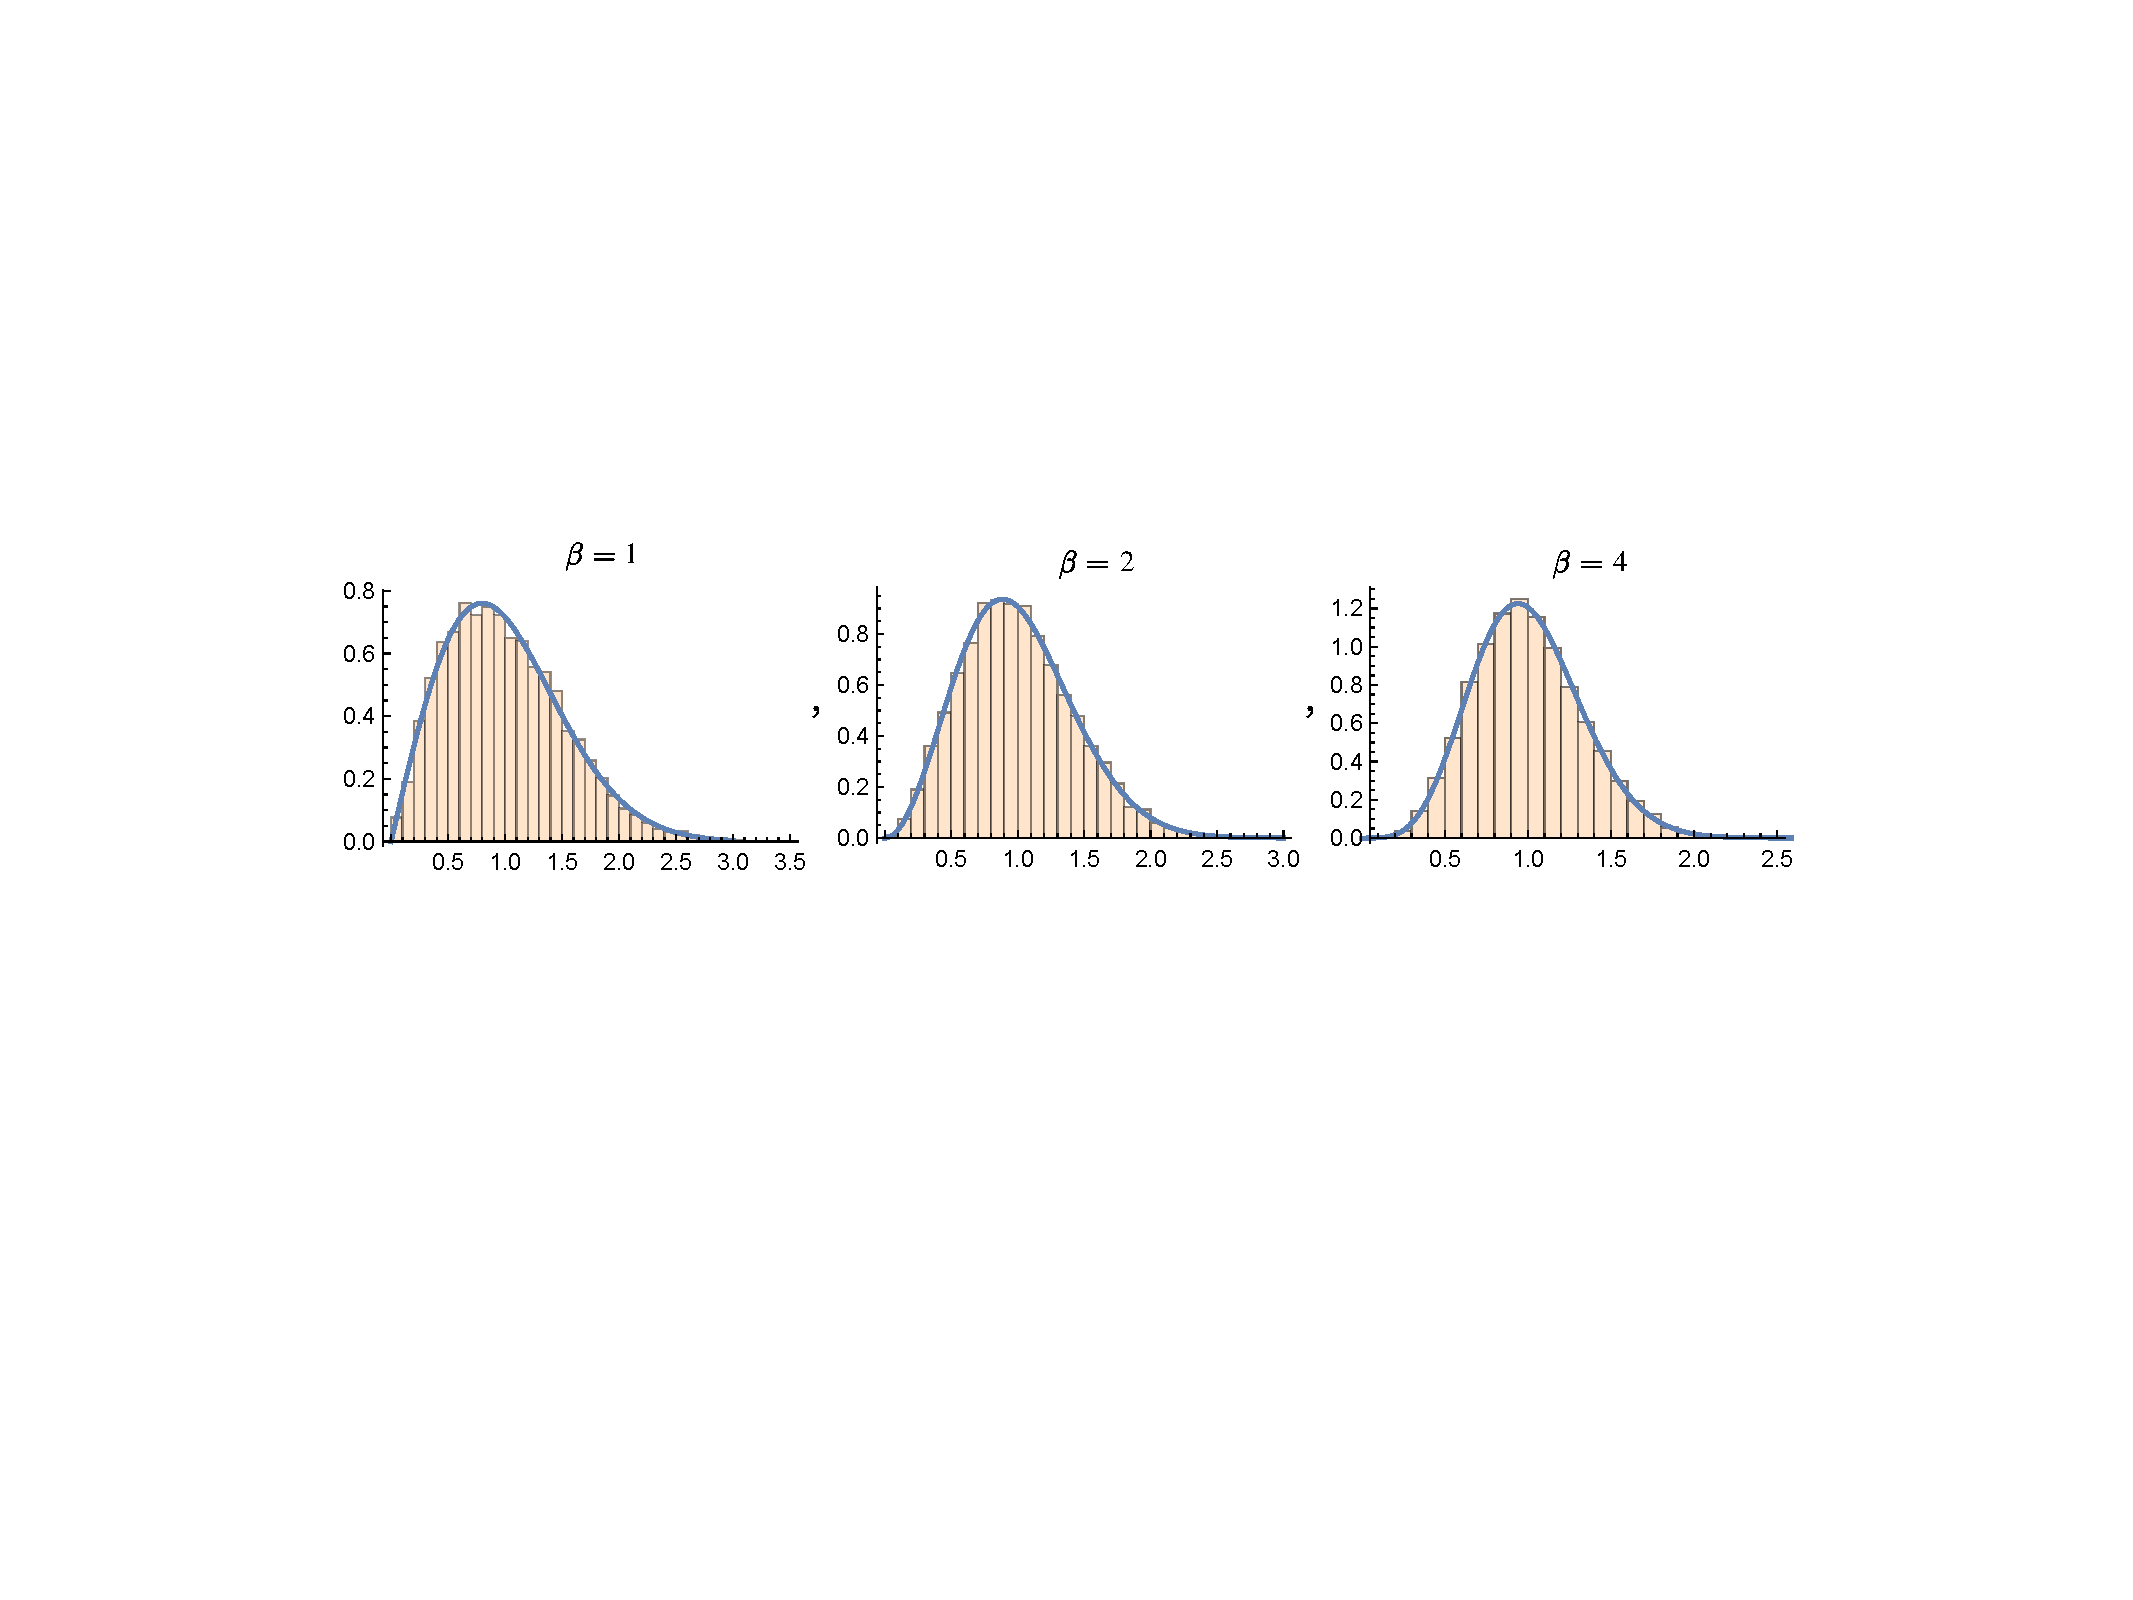
\includegraphics[width=1.05\textwidth]{figs/ensem.pdf}
	\caption{\label{fig:ensem1}The distribution of three ensembles mentioned in the text.}
\end{figure}



\begin{table}[h!]
	\centering
	\begin{tabular}{||c c c||} 
		\hline
		$\beta$ & $c_{\beta}$ & $a_{\beta}$ \\ [0.5ex] 
		\hline\hline
		%1 & $\pi s/2$ & $\pi^2 s/6$  \\ 
		%2 & $32 s^2/\pi^2$ & $\pi^2 s^2 /6$  \\
		%4 & $2^{18} s^4/3^6 \pi^3$ & $16 \pi^4 s^4/135$ 
		1 & $\pi s/2$ & $\pi/4$  \\ 
		2 & $32 s^2/\pi^2$ & $4/\pi$  \\
		4 & $2^{18} s^4/3^6 \pi^3$ & $64/9\pi$
		 \\ [1ex] 
		\hline 
	\end{tabular}
\caption{We mention the values for $c_{\beta}$ and $a_{\beta}$ for different ensembles.}
\label{table:c_and_a}
\end{table}



It is appropriate here to quote a statement by Mark Kac 
\footnote{Kac was a Polish American mathematician. His main interest was probability theory. 
He is also known apart from other things for his thought provoking question - ``Can one hear 
the shape of a drum?''} - ``That we are led here to the normal law (distribution), usually associated with random phenomena, is perhaps
an indication that the deterministic and probabilistic points of view are not as irreconcilable as they may appear at first sight''. It was later concluded that much to Wigner's own surprise, 
his guess was fairly accurate as shown and improved by Mehta \cite{MEHTA1960395} and Gaudin \cite{GAUDIN1961447}.
In fact, the field of random matrix theory is intimately related to number theory (especially the pair correlation of the zeros of the Riemann-zeta function) and this was 
observed by Montgomery and Dyson at a tea break at the Institute for Advanced Study in the 1970s. Some still believe that the proof of Riemann hypothesis lies in the
deepest secrets of random matrix theory. This belif is also the theme of the idea proposed independently by  Hilbert and P\'{o}lya who suggested that the zeros of the zeta function might be the eigenvalues of some unknown Hermitian `operator'. It is another thing that no one yet knows such an operator! We refer the reader to the excellent books \cite{Meh2004, Akemann:2011csh} for thorough introduction. 

Another major development with the matrix degrees of freedom and matrix models came with the work of 't~Hooft in 1974. By then, it was becoming clear that the correct theory of strong interactions is QCD where there are matrix degrees of freedom
which is based on $SU(3)$ gauge group. `t Hooft proposed to consider a general $SU(N)$ symmetry 
since he showed that in such limit only planar diagrams survive and calculations becomes
more tractable. In fact, this large $N$ limit was later understood to be closely related to some
description of string theory. This work brought together the idea of random matrix models
in the asymptotic limit (large matrices) to the mainstream Physics and was is fruitful till date. 
This also enabled us to study quantum gravity from a field theoretic point of view via the famous
AdS/CFT conjecture.

\begin{figure}[htbp] 
	\centering 
	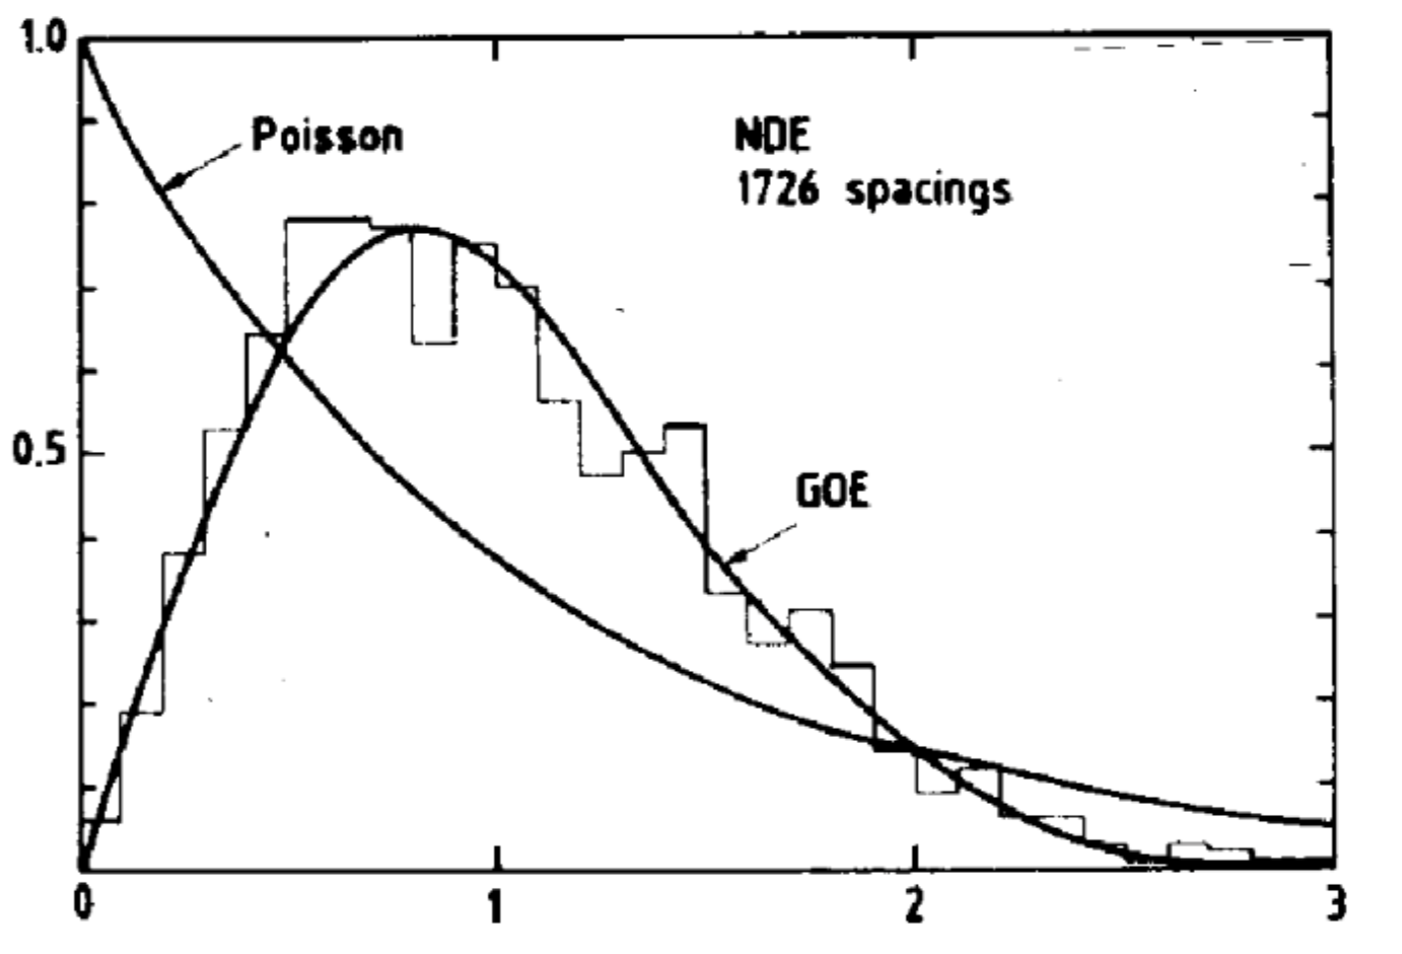
\includegraphics[width=0.55\textwidth]{figs/data_exp.png}
	\caption{\label{fig:data_exp1}The nearest neighbour spacing distribution (i.e., $P(s)$) for nuclear data. The GOE (Gaussian Orthoghonal Ensemble) and Poisson is given by solid curves. This figure is taken from - ``Fluctuation Properties of Nuclear Energy Levels and Widths : Comparison of Theory with Experiment'' by O. Bohigas, R. U. Haq, and A. Pandey}
\end{figure}
In fact, it was improved further compared to what is shown in Fig.~\ref{fig:data_exp1} in 
\cite{PhysRevLett.48.1086} 
 
 
 The plan of these notes is as follows. In ....
 There are some excellent reviews about random matrix theory, matrix integrals, and their formal aspects which are beyond the scope of this article. We refer the reader to two excellent reviews written in two different centuries \cite{DiFrancesco:1993cyw,Eynard:2015aea}


\section{Large $N$ limit of matrix valued fields} 

One of the most important ideas which has led to numerous other interesting works is the idea of large $N$ limit of field theories. 
For an extended review of many seminal papers written on this since the 't~Hooft's 1974 original article \cite{tHooft:1973alw}, we refer the reader to \cite{Brezin:1994eb}.  

\subsection{QCD and large $N$} 
As we have already pointed out, QCD has a SU(3) gauge symmetry. 
In order to understand QCD in form of some expansion, 't~Hooft introduced 
the idea of the large $N$ limit of gauge theories by considering a $SU(N)$ gauge group
and studying observables in $1/N$ expansion. We often associate more variables with greater complexity, but, 
this is not always true. There are many systems which simplify in the large $N$ limit. 
This occurs because the fields are related by a certain
symmetry which ensures that the collective behaviour of the fields becomes more constraining 
as their number increases. The resulting
coupled degrees of freedom typically look different from the Lagrangian of the initial theory. 
It was soon realized that the large $N$ limit of gauge theories is related to string theory 
as in the large $N$ limit one sums over surfaces of different genus and in 
string theory one sums over different world-sheet topologies. 
There has been numerous developments following this work which 
include factorization equations, large $N$ phase transitions, 
Eguchi-Kawai (EK) volume reductions, holography, and AdS/CFT correspondence. 
In fact, EK is a way where there is natural connection of matrix integrals to QCD. 
 At first glance in QCD, one might think that the expansion parameter is $g_{YM}$, but this is not 
true in the light of the renormalization group equations. QCD has no obvious free parameter and this creates difficulty for
perturbation theory. It is because of this problem that 't~Hooft suggested taking $N$, 
the number of colors as a parameter. The idea of large $N$ limit is not restricted just to matrix valued fields 
but exists also for vector models. Pure QCD (i.e., without fermions) 
is an example of a matrix model because the gauge fields are 
$N \times N$ matrices with $N^2$ components. 
The vector models, on the other hand, only have $N$ components. We will not discuss the 
large $N$ limit of vector models in this review because we want to only focus on matrices. 

\subsection{$\beta$ function, counting diagrams, and factorization} 

One way to think of the large $N$ limit of QCD in four dimensions is to 
look at the QCD $\beta$-function. One can then check 
whether this limit captures the defining property of QCD - a negative $\beta$ function. The perturbative 
two-loop $\beta$-function given by, 
\begin{equation} 
\label{eq:beta0}
\mu \frac{dg}{d\mu} = - \frac{1}{16\pi^2} \left (\frac{11N - 2N_{f}}{3} \right)g^3  - 
\frac{1}{256\pi^4} \left (\frac{34N^3 - 13 N^{2} N_{f} + 3N_{f}}{3N}\right)g^5 + \mathscr{O}(g^7)
\end{equation} 
This has clearly no sensible large $N$ llimit. But we can make an interesting observation. 
The left hand side of (\ref{eq:beta0}) goes as 
$ \sim g$, whereas the leading term on right for small $g$ 
goes as $ \sim g^3 N$. This convinced 't~Hooft that the 
correct limit to consider is the limit where $N \to 
\infty$ and $g^2 \to 0$ while $\lambda = g^2 N$ 
remains fixed. We often refer to $\lambda$ as the 't~Hooft coupling. 
In this limit, we get, 
\begin{equation} 
  \label{eq:beta1}
\mu \frac{d\lambda}{d\mu} = - \frac{11}{24 \pi^2} \lambda^2 -  \frac{17}{192 \pi^4} \lambda^3 + \mathscr{O}(\lambda^4) 
\end{equation} 
As can be readily seen, perturbation theory predicts that the 't~Hooft limit of QCD is an asymptotically free theory which is a good first step. It is also natural to assume that $\Lambda_{\text{QCD}}$, 
the scale parameter of strong interactions is held fixed as $N \to \infty$. One important feature of (~\ref{eq:beta1}) 
is that it is independent of number of flavors, $N_{f}$. The 
number of quark degrees of freedom is $\mathscr{O}(N)$ in the
't~Hooft limit, and hence sub-leading with respect to the number of gluon degrees of freedom, which is $\mathscr{O}(N^{2})$. 


I order to illustrate the idea of large the $N$ limit, consider the following Lagrangian with canonical normlaization:
\begin{equation}
L = -\frac{1}{2} \mathrm{Tr} \Bigg[ (\partial \Phi)^2 + g\Phi^3 + g^2\Phi^4  \Bigg] 
\end{equation} 
We can rescale $\tilde{\Phi} = g \Phi$  to get, 
\begin{equation}
L = \frac{1}{g^2} \mathrm{Tr} \Bigg[ -\frac{1}{2}(\partial \tilde{\Phi})^2 + \tilde{\Phi}^3 + \tilde{\Phi}^4  \Bigg]
\end{equation} 

As we take the planar limit, $\lambda = g_{\text{YM}}^{2} N $ remains fixed where $\lambda$ is the 't~Hooft coupling. The big field $\Phi$ which we think of as potentially including scalars $\phi$, gauge fields $A_{\mu}$ which are $N \times N$ matrices. So, the propagator $\langle \Phi \Phi \rangle$ goes as $g^2$ i.e., $\lambda/N$. In a generic matrix theory there will be $n$-point vertices such as three point and four-point interaction vertices. Both types of vertices come with the same factor of $N/\lambda$. This is the advantage of using this particular form of the Lagrangian since all vertices have same contribution. We can write the gluon propagator as,  %(shown in Fig.(\ref{fig:dl2})), 
\begin{equation}
\label{eq:gluon}
\tilde{\Phi}^{a}_{\mu b}(x) \tilde{\Phi}^{c}_{\nu d}(y) = \left ( \delta^{a}_{d}\delta^{c}_{b} - \frac{1}{N} \delta^{a}_{b}\delta^{c}_{d}\right)
\mathscr{D}_{\mu\nu}(x-y) =  \left ( \delta^{a}_{d}\delta^{c}_{b} - \frac{1}{N} \delta^{a}_{b}\delta^{c}_{d}\right)
\frac{g^2}{4\pi^2(x-y)^2}, 
\end{equation}
In some sense, the gauge field is represented by a ~`quark' with index $i$, and an ~`antiquark' with index $j$. 
The second term in the parentheses is because we need to make the gluon field traceless for the SU($N$) group we are
considering. It would not be present if we were working with U($N$). In any case, in the large $N$, 
the distinction is unimportant. Following the gluon line indices we see, the index pair at the beginning is 
the same as that at the end. In some sense, 
a gluon propagates like quark--anti-quark pair. This observation was made by 't~Hooft when he devised the \emph{double-line}  
notation. Loosely speaking, we will draw as many lines in a propagator as the indices it carries. Therefore, quark propagator 
is denoted by a single line since it carries one index, whereas a gluon propagator is drawn using double lines. 
%, see %Fig.(\ref{fig:dl2})
For $SO(N$) or $USp(N$) theories, the adjoint representation may be written as a product of two fundamental representations 
rather than a product of a fundamental and an anti-fundamental representation (like done for $SU(N)$ and $U(N)$). Since the
fundamental representation is real, there are no arrows on the propagators.\footnote{Recall that arrows fix the orientation of complex fields}. If we now introduce the standard notation where $V$, $E$, $F$ denote the vertices, edges, and faces then a vacuum diagram 
has the following dependence on $\lambda$ and $N$, 
\[ \text{diagram}(V,E,F) \sim N^{V-E+F} \lambda^{E-V}  \sim N^{\chi} \lambda^{E-V} \] 
where $\chi = F + V - E$ is assured by a theorem due to Euler\footnote{Given a surface composed of polygons with F faces, E edges and V vertices, the Euler character satisfy
	$\chi = F + V - E = 2 - 2h$, where $h$ is the number of handles (also known as `genus' ) of the surface. Since, in the large $N$ limit, the diagrams with $h = 0$ contribute the most in the large $N$ limit is also known as the planar limit (because $h=0$ means no handles like spheres)} which we note below. 
We have shown an example of this counting for two graphs in Fig.(\ref{fig:D2}) which contribute $N^2\lambda^2$ (left) and
$N^2\lambda$ (right). 

\begin{figure}[htbp] 
	\centering 
	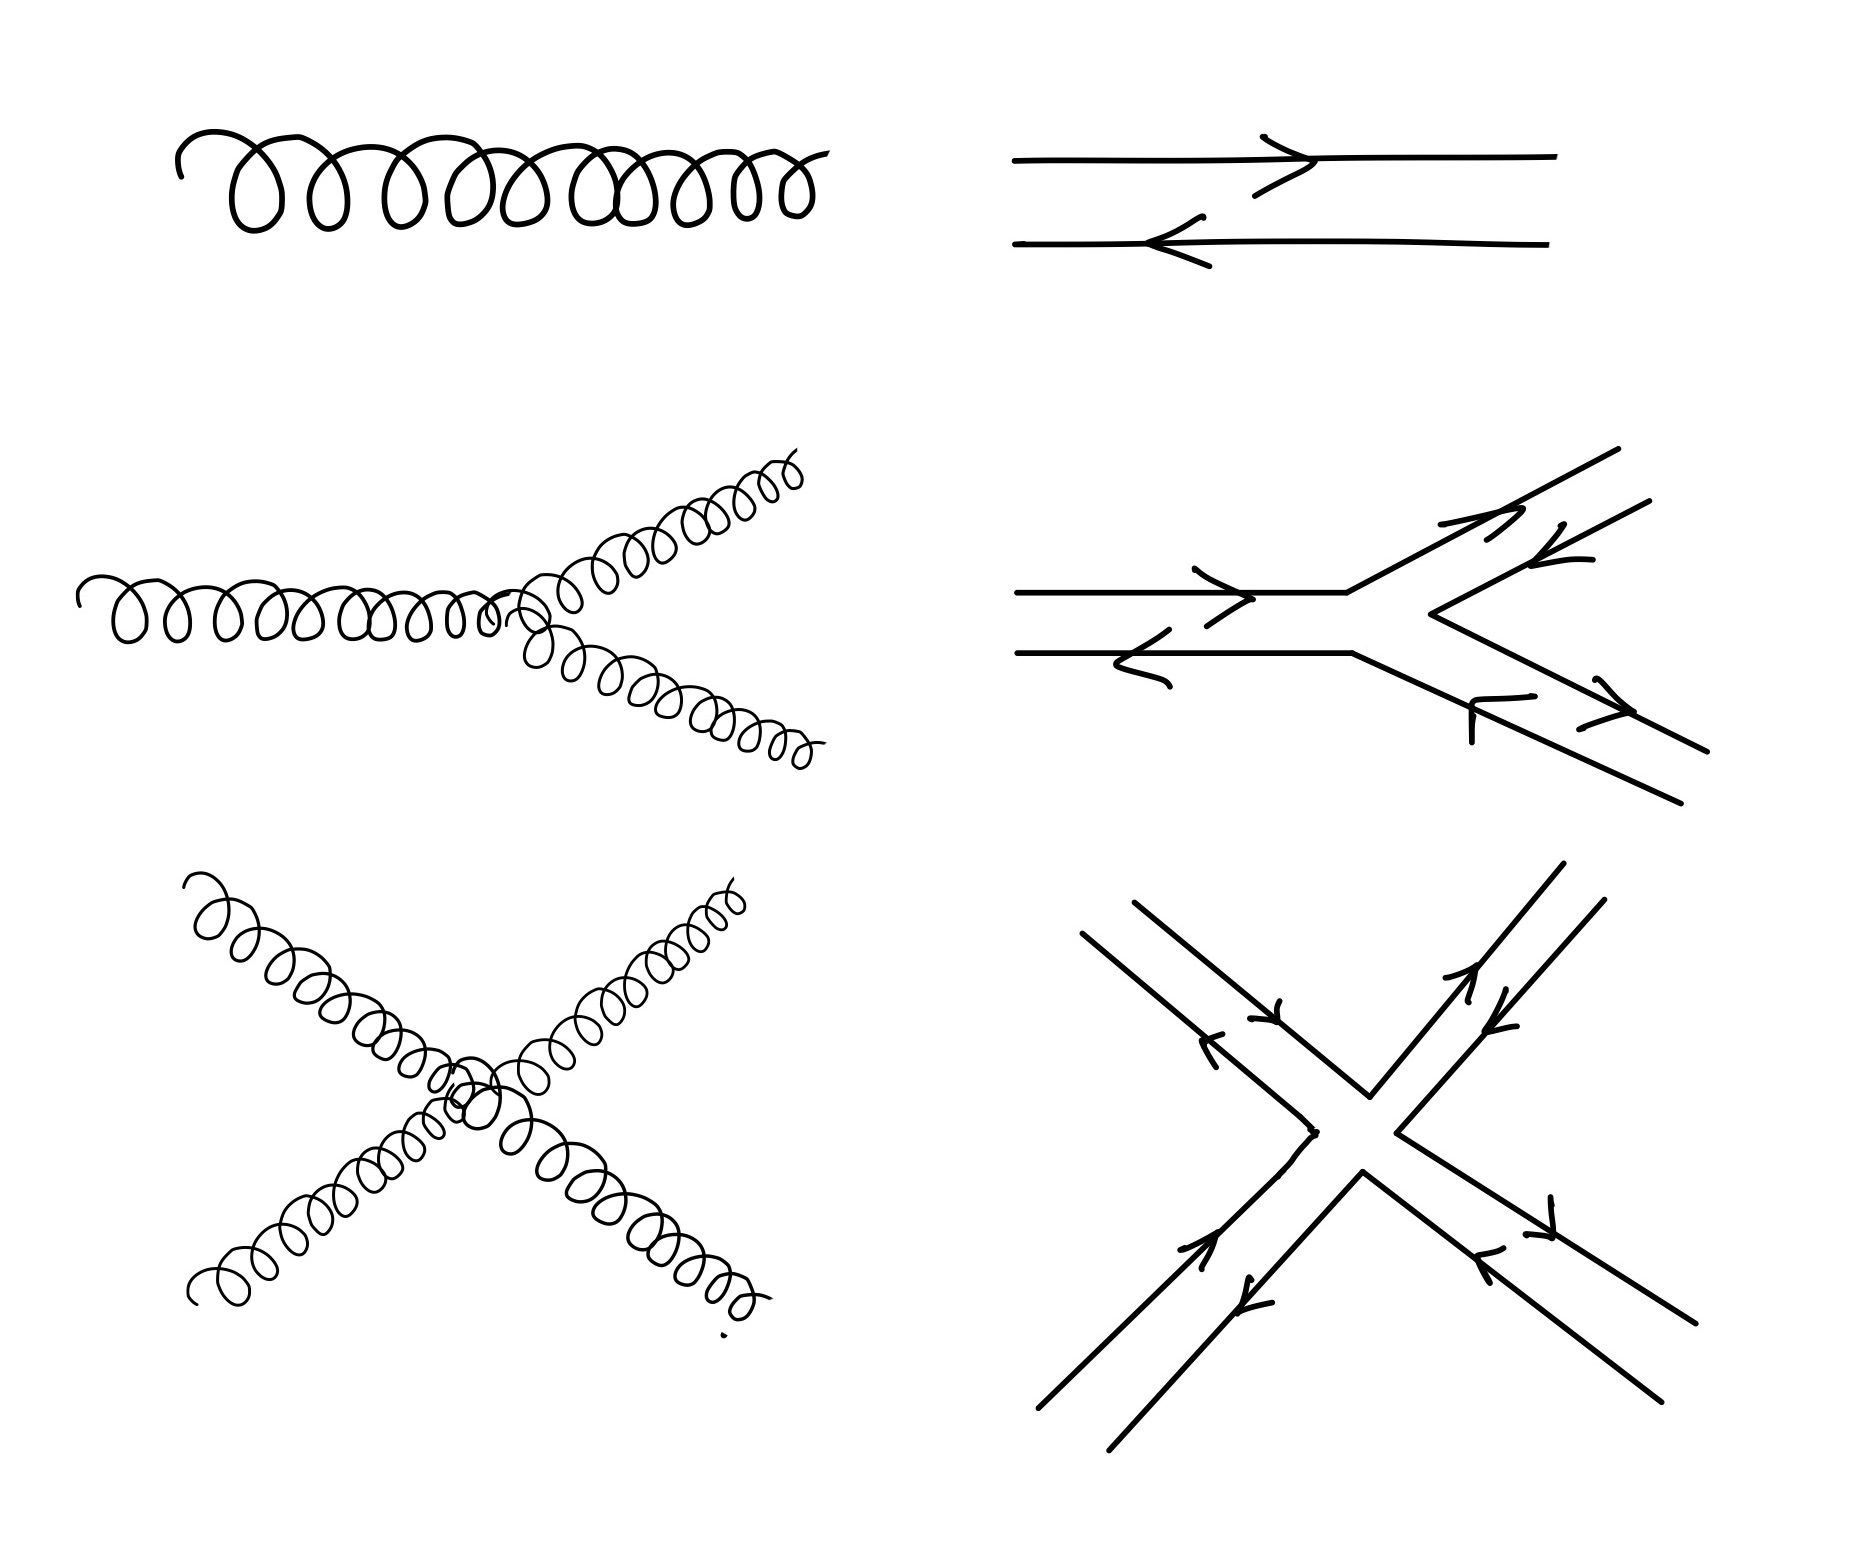
\includegraphics[width=0.55\textwidth]{figs/D1.jpg}
	\caption{\label{fig:D1}All diagrams (different $n$-point vertices) all contribute $N/\lambda$.}
\end{figure}

\begin{figure}[htbp] 
	\centering 
	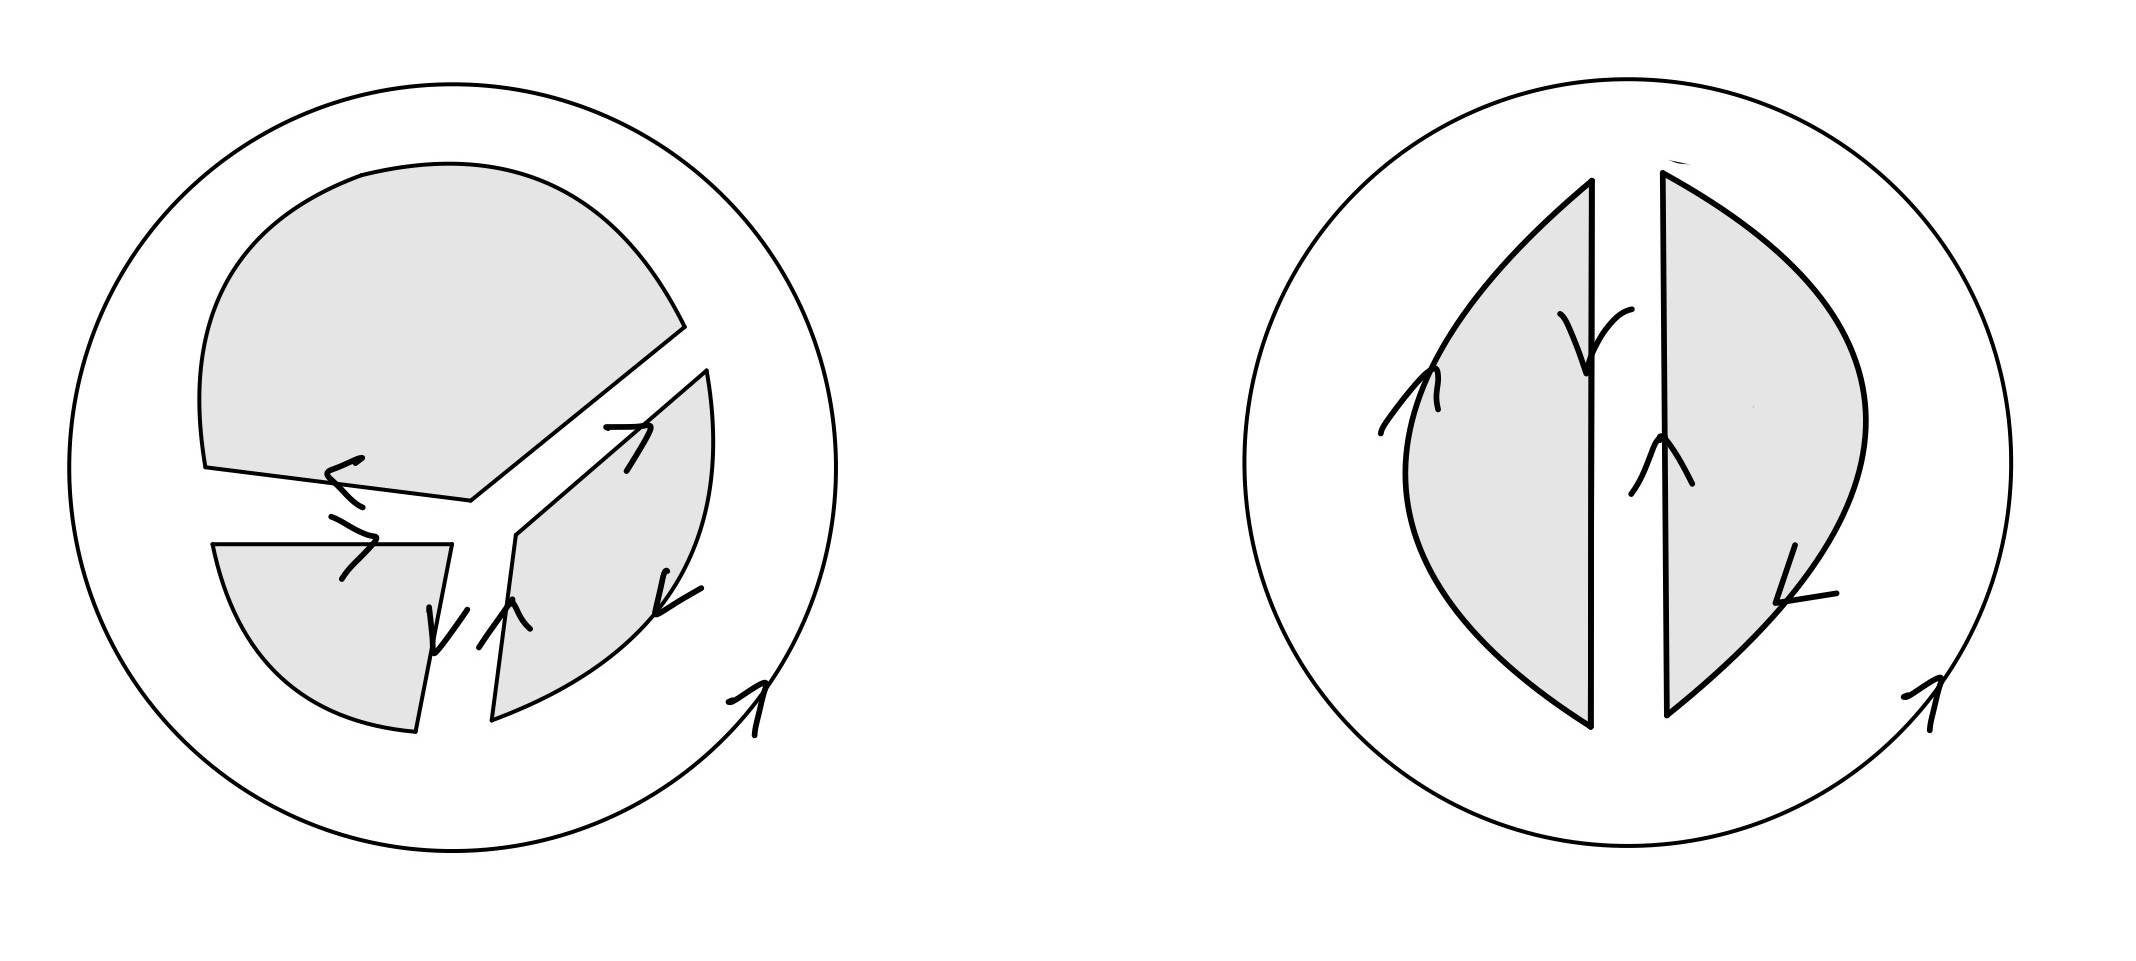
\includegraphics[width=0.55\textwidth]{figs/D2.jpg}
	\caption{\label{fig:D2}The diagram on the left contributes as $N^2\lambda^2$ while the one on the right is $N^2\lambda$ (right)}
\end{figure}
One of the remarkable features of the large $N$ limit is that it implies that the 
measure becomes concentrated on a single orbit of the gauge group. This is sometimes
also referred to as `master-field' or `master-orbit'. It is easy to show that (left as a exercise) 
if we consider a gauge-invariant observable which is properly normalized the deviation of the 
measured value from the mean is $\mathcal{O}(1/N^2)$. Mathematically, this is written for 
any two gauge-invariant operators, A and B as: 
\begin{equation}
\langle AB \rangle = \langle A \rangle  \langle B \rangle + \mathscr{O}(\frac{1}{N^2})
\end{equation}
The variance of operators vanish in this limit and there are no fluctuations. This is simplest to
for the case of pure gauge theory but can be easily extended to fermions. The bad news is that till date - no one 
has been able to calculate the master field in more than two dimensions. 


\section{Analytical solutions}

\subsection{Hermitian \& Unitary matrix models}

In these matrix models, one often needs to evaluate integrals of the form:
\begin{equation}
Z = \int \exp\Bigg[  -\mathrm{Tr} \sum V(M_{i})  -  \mathrm{Tr} \sum c_{ij}M_{i}M_{j}   \Bigg] dM_{i} dM_{j}
\end{equation}
where $M^{i}$ are $N \times N$ complex Hermtian matrices. 


In study of zero-dimensional gauge theories, we encounter these types of matrix models where the integral is over the Haar measure. These models often have interesting features in the large $N$ limit.
For ex:, in QCD, the gauge fields are elements of SU(3) and hence they are well-described in some cases by unitary matrix models. A general model is given by:



\begin{equation}
	Z = \int \exp\Bigg[  -\mbox{Tr} \sum V(U_{i})  -  \mbox{Tr} \sum c_{ij}U_{i}U_{j}   \Bigg] dU_{i} dU_{j}
\end{equation}
where $U^{i}$ are $N \times N$ unitary matrices. 

One of the well-known examples is the unitary matrix model first considered by Gross, Witten, and Wadia (GWW) around 1979. This is often known as one-plaquette matrix model. This unitary matrix model 
has deep connections to string theory in the so called `double-scaling limit' where $N \to \infty$ and $\lambda \to \lambda_{c}$ simultaneously. The requirement of this double scaling can be understood as follows: If we merely take $N \to \infty$ then we get genus zero surfaces in the expansion of the free energy. However, this would prohibit string interaction since they would imply change of genus which is not possible in that limit. In taking DSL, this problem is resolved and topological information is maintained. This model is given by : 


\begin{equation}
	Z = \int \exp \Big[- \mbox{Tr} (U + U^{\dagger})   \Big] dU
\end{equation}
This model admits exact solution for all $N$ and $\lambda$ in terms of determinant of a Toeplitz matrix. However, it is not very useful and hence this model has been studied by saddle-point methods and orthogonal polynomials (OP). We will sketch the solution using OP closely following \cite{Goldschmidt:1979hq}. 

Following the discussion in Appendix, we define the polynomial:

\begin{equation}
	P_{j}(x) = \sum_{k=0}^{j-1} b_{k} x^{k} + x^{j} 
\end{equation} 


We have to choose polynomials which are orthonormal with respect to the measure which in this case is:

\begin{equation}
	\rho(\theta) = \exp\Big[\frac{2N}{\lambda} \cos \theta \Big]
\end{equation}

and this results in:

\begin{equation}
	\int_{\-\pi}^{\pi} \rho(\theta) P_{m}(e^{i\theta}) P_{n}^{*}(e^{i\theta}) = a_{m} \delta_{mn}
\end{equation}


Let us denote $\kappa = 2N/\lambda$ then we have, 

\begin{equation}
	I_{n}(\kappa) = I_{-n}(\kappa) = \int_{-\pi}^{\pi} \rho(\theta) e^{i n \theta} 
\end{equation}
and the polynomials defined above are given by:

\begin{equation}
	P_{n}(z) = \det
	\begin{pmatrix}
		I_0 & I_1 & \cdots & I_n \\
		I_1 & I_0 & \cdots & I_{n-1} \\
		\vdots  & \vdots  & \ddots & \vdots  \\
		1 & z & \cdots & z^n 
			\end{pmatrix}
		 \frac{1}{\det [I_{i-j}]_{i,j = 1 \cdots N}}
\end{equation}
We note that the coefficients of $P_{n}(z)$ are real and hence $P_{n}^{*}(e^{i\theta}) = P_{n}(e^{-i\theta})$. It is also starightforward by expanding the determinant to see that: $a_{n} = c_{n+1}/c_{n}$ where $c_{N} = \det [I_{i-j}]_{i,j = 1 \cdots n}$ is the Toeplitz determinant. 



\begin{mdframed}[backgroundcolor=blue!3] 
	\textsc{} 
	$\bullet$ Exercise: We have derived the closed expression for the partition function of GWW model. How does this change when 
	$N$ is finite and we consider $SU(N)$ rather than $U(N)$ gauge group. \\ 
\end{mdframed} 

\begin{mdframed}[backgroundcolor=blue!3] 
	\textsc{} 
	$\bullet$ Exercise: Convice yourself using \MA that one indeed gets the Wigner semi-circle distribution when sample size is large enough for GUE ensembles. 
\end{mdframed} 

\subsection{One-matrix model: Cubic and Quartic potentials}

\subsection{Kontsevich Model}

This model is closely related to topological gravity. I 1992, 
Kontsevich proved Witte's cojecture of two-diemsioal quatum gravity 
usig matrix itegral. He cosideredd decomposition of the mpoduli space of Riemw surfaces i cells described by ribbo graphs ad the idetifyyig those gra[hs with Feyma diagrams of matrix model i the expasio of Z]

The model is given by:

\begin{equation}
	Z = \frac{\int dX \exp \Big[ -N \mbox{Tr} \Big( \frac{MX^2}{2} + \frac{iX^3}{6}\Big)\Big] }{{\int dX \exp \Big[ -N \mbox{Tr} \Big(\frac{MX^2}{2}\Big) \Big]}}
\end{equation}

\begin{equation}
	Z = \int dX \exp \Big[ -N \mbox{Tr} \Big( \frac{MX^2}{2} + \frac{iX^3}{6}\Big)\Big]
\end{equation}



Hankel and Toeplitz (i+j) versus (i-j)?


% 

\subsection{Chern-Simons and ABJM matrix models}

\subsection{Ising Model on random planar graph: Two-matrix model}

Ising Model on random graph was studied as two-matrix model first by Kazakov in 1986 and the partition function is given by:
\begin{equation}
	\label{eq:Kaz1} 
	Z = \int \mathcal{D}A \mathcal{D}B \exp N \mbox{Tr} \Bigg(-A^2 -B^2 + 2c AB -g \frac{A^3}{3} - g\frac{B^3}{3}  \Bigg)
\end{equation}

Note that this has $\mathbb{Z}_{2}$ symmetry because of 
Z being invaiant under $A \mapsto B$



\begin{equation}
	\label{eq:RIsing1} 
	Z = \int \mathcal{D}A \mathcal{D}B \exp N \mbox{Tr} \Bigg(-A^2 -B^2 + 2c AB -g_{A}e^{h} \frac{A^3}{3} 
	- g_{B}e^{-h} \frac{B^3}{3}  \Bigg)
\end{equation}

In 1986, Kazakov solved the Ising model on a random graph by \TODO{nice word} it through a two-matrix model \cite{Kazakov:1986hy}. This was later extended by Boulatov and Kazakov to admit magnetic fields \cite{Boulatov:1986sb}. We will not discuss the entire solution but will sketch the solution. They also computed the critical exponents and found different results than Onsager's case for regular square lattice. 
The exponents computed satisfied the usual Rushbrooke's law ($\alpha + 2\beta+\gamma=2$) and Widom's scaling law: $\gamma/\beta = \delta -1$. These values coincide with the  exponents obtained in a three-dimensional spherical model. This is a striking correspondence between exponents of two different models in different dimensions! In fact, after few years, while discussing the Yang-Lee edge sigularity (YLES) on dyamical graph, it was shown that an additional exponent $\sigma =1/2$ also behaved accordingly. We have listed the exponents in Table (\ref{table:crit_exp}). ggg


\vspace{10mm} 
\begin{table} 
	\begin{center} 
\begin{tabular}{|c|c|c|}
	\hline Crit. exponents & Ising model on random planar graph & Ising model on regular lattice \\
	\hline$\alpha$ & $-1$ & 0 \\
	$\beta$ & 1/2 & 1/8 \\
	$\gamma$ & 2 & 7/4 \\
	$\delta$ & 5 & 15 \\
	$\nu d$ & 3 & 2 \\
	$\gamma_{\text {str}}$ & -1/3 & - \\
	\hline
\end{tabular}
\end{center} 
	\caption{Summary of critical exponents obtained for two-dimensional Ising model on different graphs} 
	\label{table:crit_exp}
	\end{table} 



\vspace{10mm}
By turning the Z given in .... in terms of eigenvalues, we get:

\begin{equation}
	Z = \int dX dY \Delta(X) \Delta(Y)
	 \exp \Big[-N \sum_{i} (x_{i}^2 + y_{i}^{2} +2c x_{i}y_{i} + 4ge^{h}x_{i}^{4} + 4ge^{-h}y_{i}^4) \Big]
	\end{equation}

It is now clear that we would need two polynomials $P_{k}(x)$ and $Q_{j}(y)$ for this case such that their determinant matches 
$\Delta(X)$ and $\Delta(Y)$ respectively. 
These polynomials satisfy the following orthonormal condition: 

\begin{equation}
\int dx dy e^{-N V(x,y)} P_{k}(x) Q_{j}(y) = h_{k} \delta_{kj}
\end{equation}

They also satisfy several recursion relations for which the interested reader can refer to 
\cite{Boulatov:1986sb}:

\begin{equation}
	Z = \int dX dY \det[P_{r}(x_k)] \det[Q_{r}(y_k)] \exp\Big[-N \sum V(X,Y)\Big]
\end{equation}
where we have denoted $\sum_{i} (x_{i}^2 + y_{i}^{2} +2c x_{i}y_{i} + 4ge^{h}x_{i}^{4} + 4ge^{-h}y_{i}^4)$ by $V(X,Y)$. Transforiming to the eigenvalue basis of both matrices $X$ and $Y$ and using the expansion of the determinant we get:

\begin{align}
	Z &= \epsilon^{i_1 \cdots i_N} \epsilon^{j_1 \cdots j_N} \int dx_{1 \cdots N}
	dy_{1 \cdots N} P_{i_{1}}(x_1) \cdots P_{i_{N}}(x_N)
	Q_{j_{1}}(y_1) \cdots Q_{j_{N}}(y_N)
	e^{-N \sum V(x_i,y_i)} \nonumber  \\  
	&= \epsilon^{i_1 \cdots i_N} \epsilon^{j_1 \cdots j_N} \prod_{r=1}^{N} \int dx_{r} dy_{r} e^{-N V(x_r, y_r)} P_{i_r}(x_r) Q_{j_r}(y_r) \nonumber  \\  
	&=  N! \prod_{i=0}^{N-1} h_{i} 
	\label{eq:ising_r2}
\end{align}
We can define $f_{k} := h_k/h_{k-1}$ and hence 
(\ref{eq:ising_r2}) implies:

\begin{equation}
	\log Z_{N}(c,g,h) = \log N! + N \log h_0 + \sum_{k=1}^{N-1} (N-k) \log f_{k} 
\end{equation}
One is usually interested in computing the quantity (the subscript `pc' denotes planar/continuum limit i.e., $ N \to \infty$):
\begin{equation}
	F_{pc} = \frac{1}{N^2} \log\Bigg( \frac{Z(c,g,h)}{Z(c,0,0)}\Bigg) = \frac{1}{N} \sum_{k=1}^{N-1} \left(1 - \frac{k}{N} \log \Big(\frac{f_k}{f_{k,0}}\Big)\right)
\end{equation}


%\subsection{Matrix model for Ising Model on random graph in a magnetic field}

\subsection{General $p$-matrix open chain}








This model can easily be solved using the method of resolvent as explained in detail in \cite{DiFrancesco:1993cyw, Marino:2004eq} and first solved in the 
famous BIPZ \cite{Brezin:1977sv} paper. 
Consider a potential $V(y)$, 
%\begin{equation}
%V(y) = -\frac{y^2}{2} + \frac{gy^4}{4} + g^2 \zeta  %\frac{y^6}{6} 
%\end{equation}
and assume that the eigenvalues have single cut in the interval $ C = [-a,a]$ and a resolvent, 
\begin{equation}
G(x) = \int_{-a}^{a} \frac{1}{2\pi i} \frac{\sqrt{x^2-a^2}}{\sqrt{y^2-a^2}} N V^{\prime}(y) \frac{1}{x-y} 
\end{equation}
Note that if the cut was instead $ C= [b,a]$ then we would have, 
\begin{equation}
G(x) = \oint \frac{dy}{2\pi i} \sqrt{\frac{(x-a) (x-b)}{(y-a)(y-b)}}  N V^{\prime}(y) \frac{1}{x-y} 
\end{equation}

\begin{align}
	Z &= \int dM e^{-\frac{N}{g} \mbox{Tr} V(M)} \\
	& = \int \prod d\lambda_{i} \Delta^2(\lambda)  e^{-\frac{N}{g} \sum V(\lambda_i)} 
\end{align}
where $\Delta(\lambda) = \prod_{i > j} (\lambda_i - \lambda_j) = \exp[\sum_{i>j} \log |\lambda_{i} - \lambda_{j}|]$ is the Vandermonde 
determinant. If we now vary above for one of the eigenvalues gives the saddle point equation , 

\begin{equation}
	\label{eq:v_saddle}
	\frac{2}{N} \sum_{j \neq i} \frac{1}{\lambda_i - \lambda_j} = \frac{1}{g} V^{\prime}(\lambda_i)
\end{equation}

It is useful to introduce the density of eigenvalues as:

\begin{equation}
	\rho(\lambda) = \frac{1}{N} \sum_{i=1}^{N} \delta(\lambda - \lambda_i)
\end{equation}


In the limit of large $N$, we can write (\ref{eq:v_saddle})
as:
\begin{equation}
	V^{\prime}(\lambda) = 2g \fint_{a}^{b} d\mu \frac{\rho(\mu)}{\lambda - \mu} 
\end{equation}
where by $\fint$ we meant the Cauchy principal value of the integral. We can write resolvent as:

(resolvent  is the Stieljes transform of the eigenvalue density)

\begin{equation}
	G(z) = 2 \fint_{-a}^{a} d\mu \frac{\rho(\mu)}{z - \mu}
\end{equation}

then we can write above as (using Sokhotski-Plemelj  theorem

%\footnote{This theorem is $\lim_{\epsilon \rightarrow0} \int_a^b\frac{f(x)}{x+i\epsilon}dx=-i\pi f(0)+ \text{PV}\int_a^b\frac{f(x)}{x}dx$, where PV is the principal value}):

\begin{equation}
	G(z \pm i \epsilon) = \fint_{-a}^{a} d\mu \frac{\rho(\mu)}{z - \mu} \mp i\pi \rho(z) 
\end{equation}

which is just: 


\begin{equation}
	G(z \pm i \epsilon) = \frac{1}{2} V^{\prime}(z) \mp i\pi \rho(z) 
\end{equation}

Once we find the resolvent, we are done and we know $\rho(z)$.  



\begin{mdframed}[backgroundcolor=blue!3] 
	\textsc{} 
	$\bullet$ Find the expected values for $\mathrm{Tr}(X^2)$ for one matrix model (1MM) with $g$ = 1.0 in the planar limit using the well-known `saddle-point' method (also sometimes `stationary-phase'). Set up this problem for a fixed $N=100$ and carry out the Monte Carlo procedure. Compare the results. The \textsc{Python} code can be found in the \TODO{Appendix}.
	You can refer to the \textsc{Mathematica} script given in the Appendix for carrying out the analytical computation.
\end{mdframed} 

%It must be noted that the one-matrix model is very special in the sense that it is exactly solvable.

\begin{mdframed}[backgroundcolor=blue!3] 
	\textsc{} 
	$\bullet$ Exercise: Derive the loop equations (aka Schwinger-Dyson equations) given below: \\ 
	\begin{equation}
		\label{eq:LE} 
		\Big< \mbox{Tr} M^{k} V^{\prime}(M) \Big> = \sum_{l=0}^{k-1} \langle \mbox{Tr} M^{l} \rangle  \langle \mbox{Tr} M^{k-l-1} \rangle
		\nonumber
	\end{equation} 
\end{mdframed} 

%\subsection{Cubic potential}

We can also consider one-matrix model with cubic interaction instead of quartic as above. There is well-known instability associated with cubic potential. The model is given by:
\begin{equation}
	V(M) = \frac{M^2}{2} + \frac{gM^3}{3}  
\end{equation}
It is only well-defined if $ g^2 \le 1/12 = 0.04811 \sqrt{3} \implies g_{c} \le 0.21935$. This is the radius of convergence of the planar perturbation series. 


Harish-Chandra-Itzykson-Zuber (HCIZ) integral:

\begin{align}
	I &= \int \mathcal{D}U \exp \Big[ \beta \mbox{Tr} (U^{\dagger}M_1 U M_2)\Big] \\ 
	& =  \Bigg(\prod_{p=1}^{N-1} p! \Bigg) ~ \frac{\det \Big(\exp \Big[\beta \lambda_{i} \nu_{j}\Big]\Big)}{\Delta(\lambda) \Delta(\nu) \beta^{(N^2 - N)/2}} 
\end{align}
with $\beta$ being a non-zero parameter and $U$ is a unitary $N \times N$ matrix. 


We now give a simple proof of HCIZ integral formula. 

Wd can do a character expansion as follows:

\begin{equation}
	\label{eq:HCIZ_1} 
	\exp\left[\beta \mbox{Tr} (M_{1}UM_{2}U^{\dagger})\right]  = \sum_{r} \alpha_{r}(\beta) \chi_{r}(M_{1}UM_{2}U^{\dagger})
\end{equation}
where we have assumed that both $M_1$ and $M_2$ belong to the group algebra.
We can juse two orthogonality conditions given by:
\begin{equation}
	\int dU~\chi_{r}(U) \chi_{r^{\prime}}(U) = \delta_{r r^{\prime}} 
\end{equation}
and, 
\begin{equation}
	\label{eq:U_ortho} 
	\int dU~U^{r}_{\sigma\beta} ~ U^{* ~ r^{\prime}}_{\gamma\delta} = \frac{1}{d_{r}} \delta_{r r^{\prime}} \delta_{\sigma \gamma} \delta_{\beta \delta}
\end{equation}
Using (\ref{eq:U_ortho}) in (\ref{eq:HCIZ_1}), we get:
\begin{equation}
	\exp\left[\beta \mbox{Tr} (M_{1}UM_{2}U^{\dagger})\right]  = \sum_{r} \frac{\alpha_{r}}{d_r} \chi_{r}(M_{1}) \chi_{r}(M_{2})
\end{equation}
Now we have to use the expansion for $\alpha$ given by:

\begin{equation}
	\alpha_{\{n_1, \cdots, n_{N}\}}(\beta) = \beta^{n_1 + \cdots + n_N} \Bigg[ 
		\prod_{i=1}^{N} \frac{(N-i)!}{(N+n_i-i)!}\Bigg]  d_{\{n_1, \cdots, n_{N}\}}(\beta) 
\end{equation}
where $d_{\{n_1, \cdots, n_{N}\}}$ is the dimension corresponding to the partition
$(n_1, n_2, \cdots , n_N )$





Weyl formula:

Let us consider representations of the $U(N)$ group which are
labeled by a partition into $N$ parts as $(n_1, n_2, \cdots , n_N )$ with $ n_1 \ge n_2 \ge \cdots n_N$. The character \footnote{it is defined as the trace of the representation matrix} of the irreducible representation corresponding to the partition $(n_1, n_2, \cdots , n_N )$ of non-negative integers can be obtained using the Weyl's formula:

\begin{equation}
	\chi_{(n_1, n_2, \cdots , n_N )}(U) = \frac{\det (\lambda_{i}^{n_j + N - j})}{\Delta(\lambda_1, \cdots \lambda_N)}
\end{equation}
where $\lambda_i$ are the eigenvalues of the $U$ matrix in the fundamental representation and $\Delta(\lambda_1, \cdots \lambda_N)$ is the well-known 
Vandermonde determinant. 






\begin{mdframed}[backgroundcolor=blue!3] 
	\textsc{} 
	$\bullet$ Exercise: Show that $\det(V) = \prod_{i<j} (\lambda_i - \lambda_j)$ where $V$ is given by: 
	\begin{equation*}
		V = 
		\begin{pmatrix}
			1 & \lambda_1 & \lambda_{1}^{2} & \cdots & \lambda_{1}^{N-1} \\
			1 & \lambda_2 & \lambda_{2}^{2} & \cdots & \lambda_{2}^{N-1} \\ 
			\vdots  & \vdots  & \ddots & \vdots  \\
			1 & \lambda_N & \lambda_{N}^{2} & \cdots & \lambda_{N}^{N-1} 
		\end{pmatrix} = \lambda_{i}^{j-1} 
	\end{equation*}
	
\end{mdframed} 



It is now easy to show that we get the HCIZ formula. The interested reader can refer  \cite{Balantekin:2000vn} for more details. 


Darboux's theorem is a theorem in differential forms and 
a major theorem in symplectic geometry. 
Suppose that $\omega$  is a differential 1-form on an $2l$ dimensional manifold, such that $d \omega$ has constant rank $p$. Then if $ \omega \wedge (d\omega)^p = 0 $ everywhere, we can find a local coordinates so that 

\begin{equation}
	\omega = \sum_{i=1}^{l} dp_{i} \wedge dq_{i}
\end{equation}


\begin{mdframed}[backgroundcolor=blue!3] 
	\textsc{} 
	$\bullet$ Exercise: Show that by using saddle point approximation, following holds:
	\begin{equation*}
	I(\alpha) = \lim_{\alpha \to 0} \int_{-\infty}^{\infty} e^{-\frac{1}{\alpha}f(x)} ~dx = \sqrt{\frac{2\pi \alpha}{f^{\prime\prime}(x_{0})}} e^{-f(x_{0})/\alpha} 
	\end{equation*}
	
	Find the terms which are of $\mathcal{O}(\alpha)$ by doing little more work and show that:
	
	\begin{equation*}
	I(\alpha) = \int_{-\infty}^{\infty} e^{-\frac{1}{\alpha}f(x)} ~dx = \sqrt{\frac{2\pi \alpha}{f^{\prime\prime}(x_{0})}} e^{-f(x_{0})/\alpha} \Bigg[1 + 
	\Big[ \frac{5}{24} \frac{(f^{\prime\prime\prime})^2}{(f^{\prime\prime})^3} - \frac{3}{24} \frac{f^{\prime\prime\prime\prime}}{(f^{\prime\prime})^2}\Big] \alpha + \mathcal{O}(\alpha^{2})\Bigg]
	\end{equation*}
	
	
\end{mdframed} 




\subsection{Open $p$-matrix chain model}

The general $p$-matrix model chain was first considered in \cite{Chadha:1980ri} 
\begin{equation}
\label{eq:Mehta1} 
Z_{p}(g,c,\kappa) = \int \mathcal{D}M_{1} \cdots  \mathcal{D}M_{p} \exp \mathrm{Tr}\Bigg(\sum_{i=1}^{p} -M_{i}^2  - g M_{i}^{4} + c \sum_{i=1}^{p-1} M_{i}M_{i+1} 
+ \kappa M_{p}M_{1} \Bigg)
\end{equation}
Now we can set $p=3$ to get the action: 
 \begin{equation}
\label{eq:Mehta2} 
S(g,c,\kappa) = N \mathrm{Tr}\Bigg(\sum_{i=1}^{3} X_{i}^2  + \sum_{i=1}^{3} g X_{i}^{4} - c \sum_{i=1}^{2} X_{i}X_{i+1} 
- \kappa X_{3}X_{1} \Bigg)
\end{equation}

\begin{mdframed}[backgroundcolor=blue!3] 
	\textsc{} 
	$\bullet$ Exercise:  Set up the action for this three-matrix model chain problem and implement the HMC algorithm. Explore the limit when the chain is open i.e., $\kappa=0$ and when $c = \kappa$. Comment on the observation you make. 
\end{mdframed}



\section{Numerical solutions} 

There is only a selected list of analytically solvable matrix models in the planar limit. This inevitably brings 
the thought of attempting numerical solutions. Unfortunately, even here, there are not many methods 
which one can use. In fact, there only comes two methods to mind with the second method barely few years old. 
This clearly signals the fact that there still remains lot of work to be done in devising new numerical 
methods to solve matrix models. The most frequently used method is Monte Carlo (MC) but that has its own problems. 
The newly introduced numerical bootstrap method has already been used to solve several matrix models \cite{Anderson:2016rcw,Lin:2020mme,Han:2020bkb,Kazakov:2021lel} but the extension to matrix models with more than two matrices i.e., 3-matrix commutator type models or IKKT models seems difficult at the moment. This is related to the fact that with more matrices, the loop equations which become highly non-linear are difficult to handle.
In these notes, we will mostly focus on MC methods since as of this writing bootstrap methods have not been able to access or constrain matrix models with more than two matrices. However, we want to explain the bootstrap solution for the case of one matrix model as first shown by \cite{Lin:2020mme} for the interested reader. For detailed exposition, we refer the reader to the references above. We hope that this `yet' small section on bootstrap methods would be extended in later versions of these notes as more results accumulate in coming years. 

\subsection{Numerical bootstrap}

The basic idea of bootstrapping matrix models depends on the 
positivity (positive-definiteness) of the bootstrap matrix which we refer in what follows 
by $\mathcal{M}$. For the case of one matrix model with a potential $V(X)$ given by: 
\begin{equation}
    V(X) = \frac12 X^2 + \frac{g}{4} X^4, 
\end{equation}
it is straightforward to show that the odd moments of X i.e., $ t_{n} = \mbox{Tr} X^n = 0$ for odd $n$
while the even moments (of order greater than two) are all related to $t_{2} = \mbox{Tr} X^2/N$. This renders the 
model simple to bootstrap since there is no growth of words (combination of matrix or matrices!)
since all non-zero $t_{n}$ can be related to $t_{2}$. 
\begin{mdframed}[backgroundcolor=blue!3] 
	\textsc{} 
	$\bullet$ Exercise: Use loop equations and show that it is possible to write $t_{4}, t_{6}, t_{8}$ in terms of $t_{2}$. Also check this using either \MA or \PY [see Appendix for codes] 
\end{mdframed} 
If we consider positive constraints that can be derived from $\langle \mbox{Tr}(\Phi^{\dagger}\Phi) \rangle \ge 0 $
where $\Phi$ is superposition of matrices which for one matrix model is 
$ \Phi = \sum_{k} \alpha_{k} M^{k}$. This condition is equivalent to positive definite nature of
$\mathcal{M} \succeq 0 $ where $ \mathcal{M}_{ij} = \langle \mbox{Tr} M^{i+j} \rangle$. 
We can only enforce subset of these constraints. For example, it was sufficient to 
access positive definite nature of $\mathcal{M}_{6 \times 6} \succeq 0 $ and sub-matrices 
to get to the exact solution in the original article \cite{Lin:2020mme}. 
For example, $\mathcal{M}_{2 \times 2}$ is given by:
\begin{equation}
	\mathcal{M}_{jk} = 
	\begin{pmatrix}
		t_{2j} & t_{j+k}  \\
		t_{j+k} & t_{2k}  
	\end{pmatrix}  \succeq 0
\end{equation}
In this case, solving the model just means finding the bounds on $t_{2}$ since all others can then be calculated (see the exercise above). 

Following this work, a two matrix quantum mechanics 
model (in 0+1-dimensions) was solved using similar techniques. 
The results obtained were shown to be consistent with MC results. 
In this work, the Hamiltonian considered was given by:
\begin{equation}
H = \mbox{Tr} \Big( P^2 + X^2 + \frac{g}{N} X^4 \Big)
\end{equation}
and corresponding to the trial operators up to length (L) = 2, 
they considered $ \mathbb{I}, X, X^{2}$ and $P$. The bootstrap matrix
of size $2^L \times 2^L$ which should be positive definite is constructed as:

\begin{equation}
	\mathcal{M} = 
	\begin{pmatrix}
		\langle \mbox{Tr}\mathbb{I} \rangle & \langle \mbox{Tr} X^2 \rangle & 0 & 0 \\
		\langle \mbox{Tr} X^2 \rangle & \langle \mbox{Tr} X^4 \rangle  & 0 & 0 \\ 
		0 & 0 & \langle \mbox{Tr} X^2 \rangle & \langle \mbox{Tr} XP \rangle \\
		0 & 0  & \langle \mbox{Tr} PX \rangle & \langle \mbox{Tr} P^2 \rangle
	\end{pmatrix}  \succeq 0
\end{equation}
They considered bootstrap matrices up to $L=4$ and observed
convergence to the expected result. 
For the case of two-matrix quantum mechanics, the convergence
was found to be slow but consistent with results expected using 
Monte Carlo results and bounds from Born-Oppenheimer wavefunction. 

Another two-matrix integral model given by the action 
(\ref{eq:GHM1}) was recently solved \cite{Kazakov:2021lel}. 
In this work, authors used relaxation bootstrap methods for 
$\Lambda=11$ (determining the length of largest words considered)
to constrain the moment to five decimal places. They obtained $\mathrm{Tr}X^2/N = t_2$ 
to be bounded between $ 0.421783612 \le t_2 \le 0.421784687$ while $\mathrm{Tr}X^4/N = t_4$ 
between $0.333341358 \le t_4 \le 0.333342131$.
This model in more detail 
and its corresponding solution using MC methods will be discussed in 
\TODO{SECTIO ---}



\subsection{Monte Carlo method}

The numerical method which is state-of-the-art in classical computations 
of matrix models and quantum field theories in general is the Monte Carlo approach.
For higher-dimensional models, one starts with the lattice formulation which reduces the 
path-integral introduced by Feynman into many ordinary integrals. But even for a simple
gauge theory like $\mathbb{Z}_{2}$ in four dimensions this is not practical to evaluate. 
The fact that we need to do so many integrals suggests that may be some statistical 
interpretation and this is where the basic idea of Monte Carlo comes in. It selects the 
configuration which dominates the path integral and then ignores the rest of the available
phase space.In that way one constructs a chain of configurations which can lead to the 
required distribution. Metropolis-Hastings algorithm and Hamiltonian/Hybrid Monte Carlo (HMC) 
are two frequently used methods which 
can generate a Markov chain and lead to unique stationary distribution. 
We will here focus on the latter since that has now become the state-of-the-art in 
various numerical computations. This method was introduced in 1987 by 
Duane, Kennedy, Pendleton, and Roweth who put together the ideas from
Markov chain Monte Carlo (MCMC)\footnote{MCMC originated in the seminal paper of Metropolis et al
\TODO{cite}, where it was used to simulate the state distribution for a system of ideal molecules.} 
and molecular dynamics (MD) methods. For a detailed review about HMC and its extension to
rational HMC which is required for fermions, the interested readers can 
consult the Refs. \cite{Hanada:2018fnp}. The two basic parts of HMC are: 
a) Use of integrator to evolve and propose a new configuration, b) accept or reject
the proposed configuration.  


\subsubsection{Leapfrog integrator and Metropolis step}

The leapfrog method is used to numerically integrating differential equations. This is a second-order method in the sense that energy non-conservation depends on square of step-size used. This method is `symplectic', i.e., it preserves the area of the phase space. 
\begin{figure}[htbp] 
\centering 
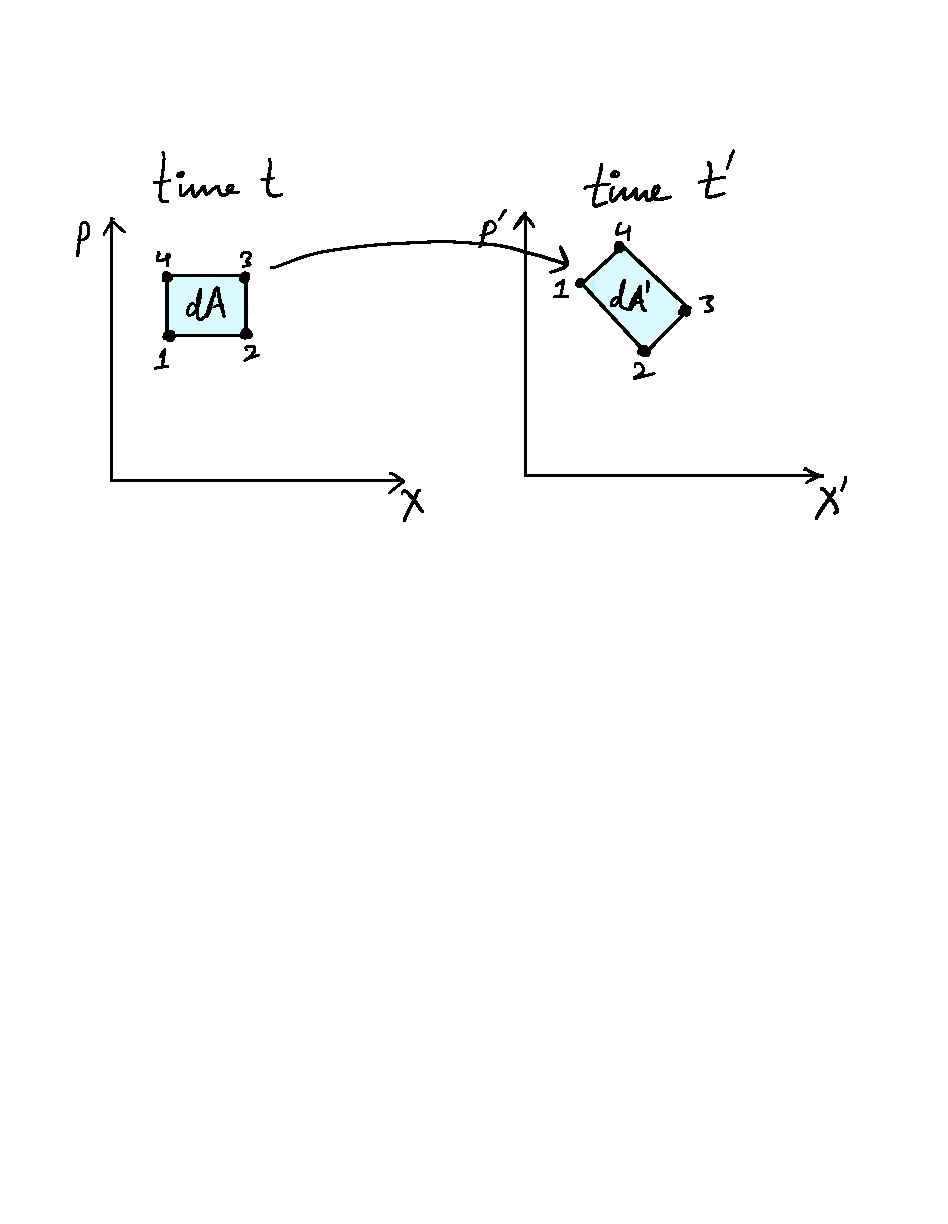
\includegraphics[width=0.75\textwidth]{figs/PSP.pdf}
\caption{\label{fig:F1}A representation of conservation of phase space area. This is also referred to as `Liouville theorem. it asserts that under evolution of the system, it may change the shape of the shaded region but not the volume since probability has to be conserved. }
\end{figure}
We can intuitively understand this as follows: 
Consider a rectangular region of area $dA$ as shown below in Fig. (\ref{fig:F2}). The four corners at time $t$ are denoted by $(x, p), (x + dx, p), (x, p + dp), (x + dx, p + dp)$. At some later time $t^{\prime}$, this will change to form corners of some quadrilateral 
as shown with area $dA^{\prime}$. 
The Liouville's theorem\footnote{This statement of Liouville theorem is closely related to detailed balance condition which says that in equilibrium there is balance between any two pairs of states i.e., equal probability.} states that the areas are equal, i.e., $dA = dA^{\prime}$. 
Using this idea we can easily prove an important equality used to check various lattice computations employing symplectic algorithms. The basic steps of the algorithm are as follows:

\begin{itemize}
	\item $X_{i}(\delta \tau/2) = X_{i}(0) + P_{i}(0)\delta \tau/2$
	\item Now several inner steps where $n =  1 \cdots (N-1)$
	\subitem $P(n \delta \tau) = P((n-1) \delta \tau) - f_{i}((n-\frac{1}{2}) \delta \tau) \delta \tau$ 
	\subitem $X((n + 1/2) \delta \tau) = X((n - 1/2) \delta \tau) + P_{i}(n \delta \tau) \delta \tau$
	\item $P(N \delta \tau) = P((N-1) \delta \tau) - f_{i}((N-\frac{1}{2}) \delta \tau) \delta \tau$ 
	\item $X(N \delta \tau) = X((N - 1/2) \delta \tau) + P_{i}(N \delta \tau) \frac{\delta \tau}{2}$ 
	
\end{itemize} 


% Page 296 of https://www.google.ca/books/edition/Molecular_Dynamics_On_Parallel_Computers/AWnVCgAAQBAJ?hl=en&gbpv=1&dq=detailed+balance+liouville+theorem&pg=PA296&printsec=frontcover
% Goodstein - States of Matter book
    \begin{mdframed}[backgroundcolor=blue!3] 
    \textsc{} 
    $\bullet$ Exercise: Show that if a symplectic integrator is used, then $ \langle e^{-\Delta H} \rangle = 1$. Check this this also holds in any given HMC simulation within errors. 
    \end{mdframed} 
    
%Because it is time-reversible, and because it is symplectic, leapfrog integration 
%is used in Hamiltonian Monte Carlo.

In the last step of HMC, a Metropolis test is carried out to accept or reject the proposed
configuration. Suppose we start from the configuration $X$ of a one matrix model 
which is a $N \times N$ matrix and carry out the leapfrog part with some parameters and obtain a new configuration 
$X^{\star}$. The test then computes: \texttt{$\text{min.}(1, e^{-\Delta H})$} and generates 
a random number between $r \in [0,1]$. The new configuration is rejected 
if \texttt{$\text{min.}(1, e^{-\Delta H}) < r$} otherwise accepted. 

\subsubsection{Random number generator}  
%%%%%%%%%%%%%%%%%%%%%%%%%%%%%%%%%

We will now discuss how to generate momentum matrices at the start of the leapfrog method taken from a Gaussian distribution. Suppose we have two numbers $U$ and $V$ taken from uniform distribution i.e., (0,1)  and we want two random numbers with probability density function $p(X)$ and $p(Y)$ given by:
\begin{equation}
	p(X) = \frac{1}{\sqrt{2\pi}} e^{-X^2/2} 
\end{equation}
and, 
\begin{equation}
	p(Y) = \frac{1}{\sqrt{2\pi}} e^{-Y^2/2} 
\end{equation}


Since $X$ and $Y$ are independent sets:

\begin{equation}
	p(X,Y) = p(X) p(Y) = \frac{1}{2\pi} e^{-R^2/2} = p(R, \Theta) 
\end{equation}

where $R = X^2 + Y^2$. This then means that we can identify the below:

\begin{equation}
	U = \frac{\Theta}{2\pi} 
\end{equation}


and, 

\begin{equation}
	V = e^{-R^2/2} \implies R = \sqrt{-2 \log(V)} 
\end{equation}

This then immediately means, 

\begin{align}
	X &= R \cos \Theta = \sqrt{-2 \log(V)} \cos(2 \pi U) \\
	Y &= R \sin \Theta = \sqrt{-2 \log(V)} \sin(2 \pi U)
\end{align}

The code to implement this is given below: 

\vspace{10mm} 
\noindent $\ddagger$ Sample code of random number generator
\begin{mdframed}[backgroundcolor=cyan!1] 
\begin{lstlisting}[language=Python]
def box_muller():  
# Basic form (alt: polar form) of Box-Muller random number generator for pairs of 
# independent, standard, normally distributed (mean=0, sigma=1) 
# given a source of uniformly distributed random numbers in (0,1)
# p, q have weights exp(-p^2/2)/sqrt(2pi) and exp(-q^2/2)/sqrt(2pi) respectively. 

    PI = 2.0*math.asin(1.0);    
    r = random.uniform(0,1)
    s = random.uniform(0,1)
    x = np.sqrt(-2.0*np.log(r)) * math.sin(2.0*PI*s)
    y = np.sqrt(-2.0*np.log(r)) * math.cos(2.0*PI*s)
    return x,y
\end{lstlisting}
\end{mdframed} 

It is easy to check that it indeed generates a 
sGaussian distribution as shown in Fig.\ref{fig:RN}. 


\begin{figure}[htbp] 
	\centering 
	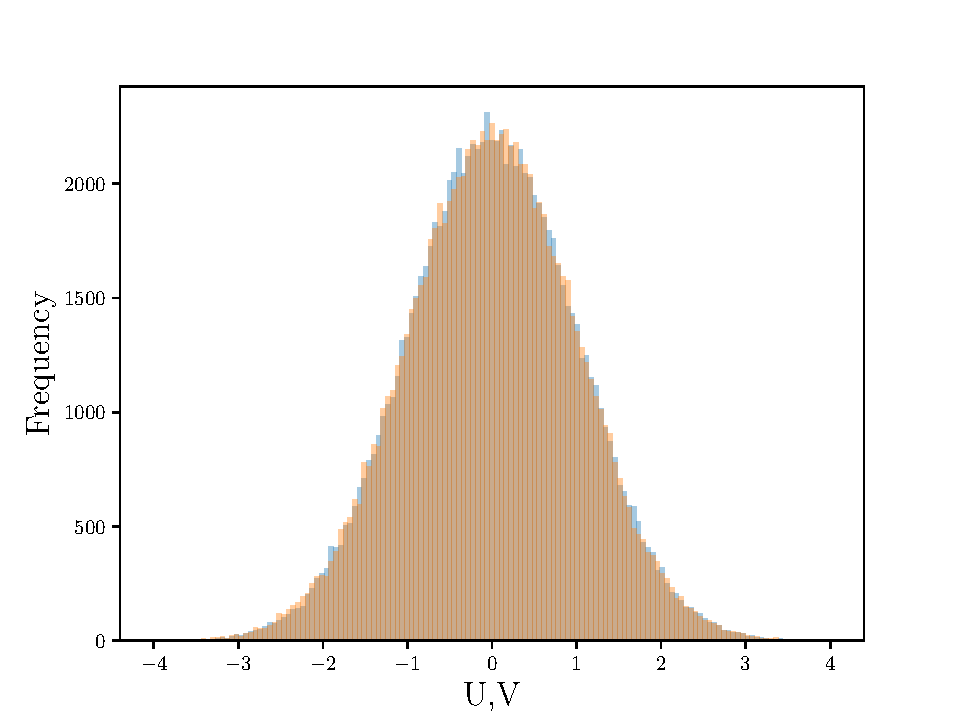
\includegraphics[width=0.75\textwidth]{figs/testRN.pdf}
	\caption{\label{fig:RN}In the limit of large sample size, it tends to Gaussian with mean zero and $\sigma=1$.}
\end{figure}


%%%%%%%%%%%%%%%%%%%%%%%%%%%%%%%%%

\subsubsection{Autocorrelation and errors} 

It is well-known that in any given Markov chain, the new states (i.e., configurations) can be highly correlated to previous ones. In order to ascertain that the measurement of an observable $\mathcal{O}$ is not affected by correlated configurations, it is essential for proper statistical analysis to know the extent to whicht they are
correlated. In this regard, it is important to measure
the autocorrelation time $ \tau_{\rm{auto}}$ which measures the time it takes for two measurements to be considered independent of each other. So, if we generate $L$ configurations, then actually only $L/\tau_{\rm{auto}}$ are useful for computing averages.
%$\tau$ is often given by Kubo formula which is 
We define autocorrelation function of observable $\mathcal{O}$ as:
 
 \begin{equation}
 	C(t) = \frac{\langle \mathcal{O}(t_0) \mathcal{O}(t_0 + t) \rangle - \langle \mathcal{O}(t_0)\rangle \langle \mathcal{O}(t_0 + t) \rangle}{\langle \mathcal{O}^2(t_0)\rangle - \langle \mathcal{O}(t_0)\rangle^{2}}
 \end{equation}
The behaviour of $C(t)$ is $\sim \exp(-t/\tau_{\rm{auto}})$ as $ t \to \infty$. This is called exponential autocorrelation time. We can also compute something which is called `integrated autocorrelation time' defined as:
\begin{equation}
	\tau_{\rm{auto}}^{\rm{int.}} = \frac{\sum_{t=1}^{\infty} \langle \mathcal{O}(t_0) \mathcal{O}(t_0 + t) \rangle - \langle \mathcal{O} \rangle^2 }{\langle \mathcal{O}^2\rangle - \langle \mathcal{O}\rangle^{2}}
\end{equation}
We can write this in terms of sum over autocorrelation function as: $\tau_{\rm{auto}}^{\rm{int.}} = 1 + \sum_{t=1}^{N} C(t)$. In general, $ \tau_{\rm{auto}}$ increases with system size, close to critical point. Once can express the statistical error in the average of $\mathcal{O}$ denoted by $\delta \mathcal{O}$ is given in terms of variance and integrated autocorrelation time as:

\begin{equation}
	\delta \mathcal{O} = \frac{\sigma}{\sqrt{N}} \sqrt{2 \tau_{\rm{auto}}^{\rm{int.}}}
\end{equation}
where we have usual definitions i.e., 
$\sigma = \sqrt{\langle \mathcal{O}^2\rangle - \langle \mathcal{O}\rangle^{2}}$ and $N$ is the number of measurements. 




\subsection{One-matrix model: Confirming exact results} 
\subsection{Matrix model closed chain solution} 
\subsection{Three-matrix Yang Mills matrix model}

\TODO{Read Badis review} 
\TODO{Add Chern-Simon term}

%\begin{itemize} 
%\item Compute the autocorrelation time for the time-series in \texttt{action.txt}
%using either \texttt{acor} or \texttt{emcee}. 
%\href{https://github.com/rgjha/TensorCodes/blob/master/2d_trg.py}
%{here}. 
%\item Explore the different ratios $r = g/\kappa$ in the 3 MM problem and think about the symmetry. 
%\item 
%\end{itemize} 


\subsection{Hoppe's matrix model}

This model was first introduced by Hoppe in 1982 and solved later by 
Kazokov-Kostov-Nekrasov (KKN) in \cite{Kazakov:1998ji}. The partition function is given by:

\begin{equation}
Z = \int \mathcal{D}X \mathcal{D}Y \exp \Big[-N ~ \rm{Tr} (X^2 + Y^2 - g^2 [X,Y]^2) \Big] 
\end{equation}

At large values of coupling i.e., $ g \to \infty$, this model becomes commuting with 
$ [X,Y] \to 0$. The presence of commutator term in matrix models is common especially in models which have a dual gravity interpretation. 
The exact result for average action is:

\begin{equation}
	2 \langle S_{c} \rangle + \langle S_{q}  \rangle = N^2 - 1, 
\end{equation}
where $ S_{c} = -Ng^2 \rm{Tr}[X,Y]^2$  and 
$ S_{q} = N \rm{Tr} (X^2 + Y^2) $

\subsection{Generalized Hoppe's model}

We can consider a slightly more general two-matrix model which reduces to 
Hoppe's model mentioned above in a special limit. Such a matrix model generally not solvable. 
This model was considered in \cite{Kazakov:2021lel} and solved using bootstrap methods. 

\begin{equation}
\label{eq:GHM1} 
Z = \int \mathcal{D}X \mathcal{D}Y \exp \Big[-N ~ \rm{Tr} (X^2 + Y^2 - g^2 [X,Y]^2 + hX^4 + hY^4) \Big]	
\end{equation} 

For $h = 0$ it can be reduced to Hoppe's matrix model which can be solved via saddle-point analysis or through the reduction to a Kadomtsev-Petviashvili (KP) type equation. For $g = 0$ it reduces to two decoupled one-matrix models and for $g = \infty$, we have [X, Y] = 0 and it becomes an eigenvalue problem. 

We show in Fig. \ref{fig:2MM_match} obtained using Monte Carlo (MC) are 
consistent with those obtained in \cite{Kazakov:2021lel}. The shown MC 
results were obtained for $N=200$ in 445 seconds on a 2019 Macbook. 

\begin{figure}[htbp] 
	\centering 
	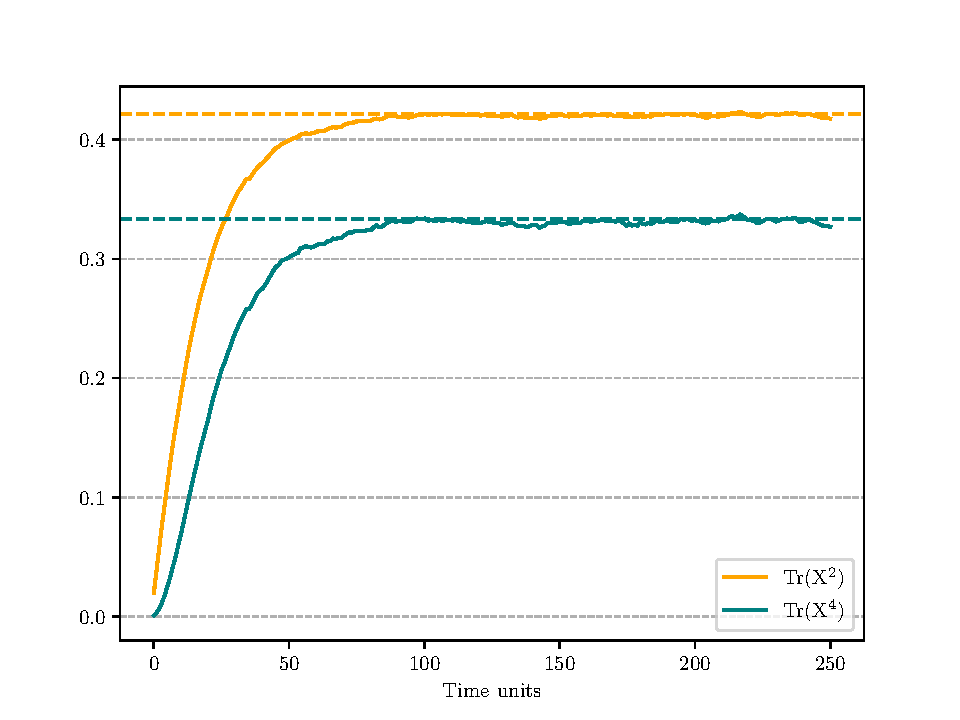
\includegraphics[width=0.75\textwidth]{figs/plot_2MM.pdf}
	\caption{\label{fig:2MM_match} We show the bootstrap results by dashed lines and MC by solid lines}
\end{figure}

\subsection{Extension of Hoppe's model to $D$ matrices}

Matrix model with $SO(D)$ invariance:

\begin{equation}
	Z = \int \mathcal{D}X_1 \cdots \mathcal{D}X_d ~
	\exp\Big[ -\sum_{i} \mbox{Tr} X_{i}^{2} + \lambda^2 \sum_{i,j} \mbox{Tr} [X_i,X_j]^{2}\Big]
\end{equation}

If we consider $X_i \mapsto (1+\epsilon) X_i$, it must leave $Z$ invariant, one arrives at:

\begin{equation}
	d(N^2 -1) = 2d \langle \mbox{Tr}X_{i}^{2} \rangle 
	-4 \lambda^2 d(d-1) \langle \mbox{Tr}[X_i,X_j]^{2} \rangle
\end{equation}

\subsection{Dimer Model: Yang-Lee singularity}

We start from Equation (4.7) in \cite{Staudacher:1989fy} 
\begin{equation}
	\label{eq:Stau0}
	Z = \int \mathcal{D}X \mathcal{D}M \exp N \mbox{Tr}\Bigg(-\frac{X^2}{2} + \frac{gX^4}{4} - \frac{M^2}{2} + g \sqrt{\zeta} MX^3 \Bigg)
\end{equation}
and then integrate out the matrix $M$ by completing the squares method to get:
\begin{equation}
	\label{eq:Stau1} 
	Z = \int \mathcal{D}X \exp N \mbox{Tr}\Bigg(-\frac{X^2}{2} + \frac{gX^4}{4} + g^2 \zeta  \frac{X^6}{2}   \Bigg)
\end{equation}
Note that if we set $\zeta=0$, this reduces to the familiar 1MM problem we solved in previous section. 

% ax^2 + bx + c -> a(x-h)^2 + k 
% where h = -b/2a and k = c - (b^2/4a)  

\begin{mdframed}[backgroundcolor=blue!3]  
	$\bullet$ Exercise: Check that \ref{eq:Stau1} follows from \ref{eq:Stau0}. 
\end{mdframed} 



\subsection{Matrix chain: Ends closed}

The matrix chain is a complicated $p$ matrix model which was first considered in \cite{Chadha:1980ri}. When the chain is connected, the model is not solvable. We use Monte Carlo methods to study this with $N=100$ which is close to the desired planar limit. 


\begin{figure}[htbp] 
	\centering 
	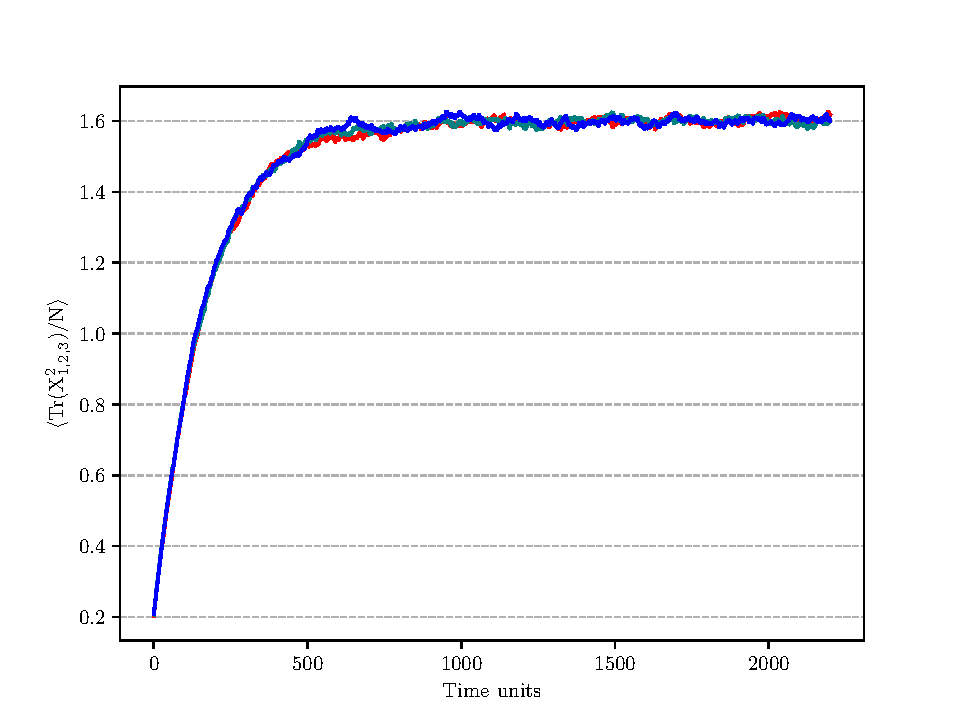
\includegraphics[width=0.75\textwidth]{figs/plot_3MM_chain.pdf}
	\caption{\label{fig:F_app1}The computed value of normalized $\mbox{Tr}(X_{1,2,3}^2)$ with MC methods when $g=1$ and $\kappa=c=1.35$. It is clear that there is a $SO(3)$ symmetry between scalars and they converge to the same value $\sim$ 1.61 for $N = 100$ we have considered.}
\end{figure}

\begin{figure}[htbp] 
	\centering 
	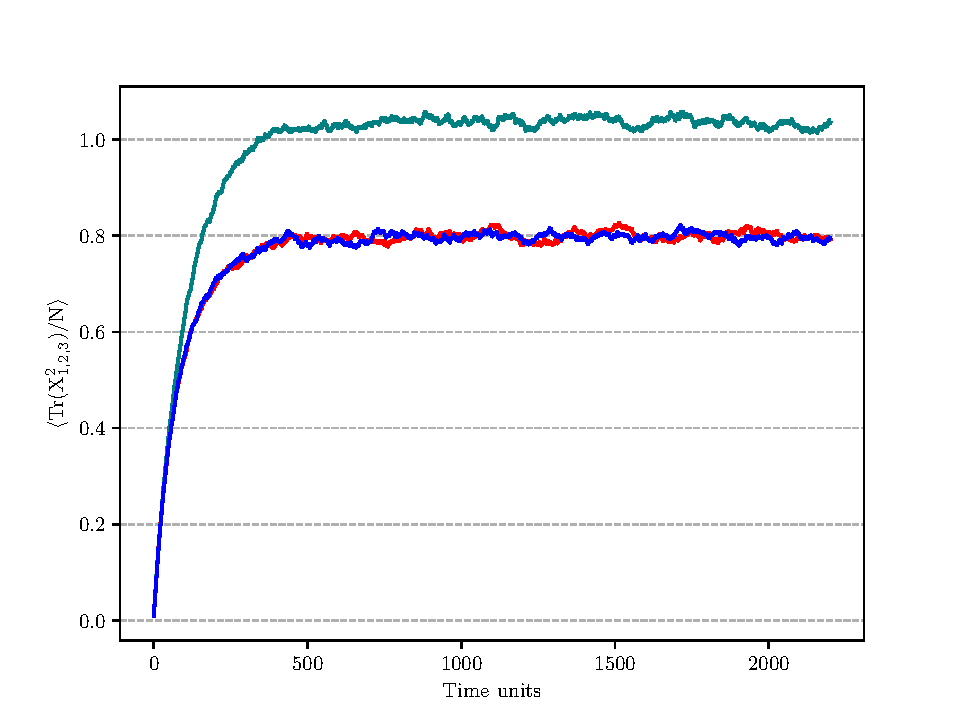
\includegraphics[width=0.75\textwidth]{figs/open_3MMC.pdf}
	\caption{\label{fig:F_app1}The computed value of normalized $\mbox{Tr}(X_{1,2,3}^2)$ with MC methods when $g=1, c=1.35, \kappa=0$. The absence of term connecting the ends results in  $SO(3)$ symmetry being broken. They converge to two sets of value $\sim 0.80$ and $\sim 1.03$ for $N = 100$.}
\end{figure}


\begin{equation}
	\label{eq:Mehta1} 
	Z_{p}(g,c,\kappa) = \int \mathcal{D}M_{1} \cdots  \mathcal{D}M_{p} \exp \mbox{Tr} \Bigg(\sum_{i=1}^{p} -M_{i}^2  - g M_{i}^{4} + c \sum_{i=1}^{p-1} M_{i}M_{i+1} 
	+ \kappa M_{p}M_{1} \Bigg)
\end{equation}

\begin{equation}
	\label{eq:Mehta2} 
	S(g,c,\kappa) = N \mbox{Tr} \Bigg(\sum_{i=1}^{3} X_{i}^2  + \sum_{i=1}^{3} g X_{i}^{4} - c \sum_{i=1}^{2} X_{i}X_{i+1} 
	- \kappa X_{3}X_{1} \Bigg)
\end{equation}

%%%%%%%%%%%%%%%%%%%%%%%%%%%%
\section{Matrix models for string theory and holography} 

\subsection{$c=1$ MQM}
One of the significant developments in the 1990s was the realization that there is a duality between a special $c=1$ matrix quantum mechnics (MQM) and two-dimensional bosonic string theory. The action for the matrix model is given by:

\begin{equation}
	Z = \int \mathcal{D} X \exp \Bigg[-\beta \int dt~\mbox{Tr} (\dot{X}^2) + V(X) \Bigg]
\end{equation}
where $t$ runs either from $-\infty$ to $\infty$ or from 0 to 2$\pi$ and $X$ is a 
$ N \times N$ Hermitian matrix. The planar graph expansion of $Z$ discretizes string worldsheet in the target space time direction $t$ while an additional spatial direction  
grows from the eigenvalue coordinate of $X$. By changing to the eigenvalue basis and introducing an antisymmetric function, it can be show that this model reduces to a fermionic problem with $N$ degrees of freedom in external potential with each `particle' behaving independently. This is in fact very surprising since we initially started with Bose particles and now ran into Fermi statistics \cite{Brezin:1977sv,Kazakov:1988ch}. 
This relation to $N$ free fermions is the foundation of the exact solubility of string theory in two dimensions \cite{Klebanov:1991qa}. 

\vspace{10mm}

\begin{mdframed}[backgroundcolor=blue!3] 
	\textsc{} 
	$\bullet$ Exercise: Show that if $\Delta(\lambda) =\prod_{i<j} (\lambda_i - \lambda_j)$, then following is true: 
	
	\[ \sum_{i} (\lambda_i)^{k} \frac{\partial^{k}}{\partial^{k} \lambda_i} \Delta =
	 \sum_{r=k}^{n-1}\frac{r!}{(r-k)!} \Delta = \frac{n (n-1) \cdots (n-k)}{k+1}
	 \Delta = k! {{n}\choose{k+1}} \Delta
	 \]
\end{mdframed} 

% https://mathoverflow.net/questions/78540/a-sum-involving-derivatives-of-vandermonde


% c[n_,k_]:=Product[(n-k+i),{i,0,k}]/(k+1); 
% d[n_,k_] := Sum[r!/(r-k)!,{r,k,n-1}]; 
% e[n_,k_] := Binomial[n,k+1] k! 


% https://web.phys.ntu.edu.tw/string/matrix/NuclPhysB311(1988_89)171_Kazakov_Migdal_RecentProgressInTheTheoryOfNoncriticalStrings.pdf

% https://arxiv.org/pdf/hep-th/0012228.pdf,

% Klebaov: https://arxiv.org/pdf/hep-th/9108019.pdf

% https://arxiv.org/pdf/hep-lat/0009030.pdf

% https://arxiv.org/pdf/hep-th/9803117.pdf

\subsection{BFSS matrix model}

The non-perturbative features of supersymmetric Yang-Mills (SYM) is thought to play a crucial role in the beyond Standard model (BSM) Physics and also in M/String theory. The non-perturbative study of string theory is based on various matrix models. Up to present, two kinds of non-perturbative formulation of
M/string theory are developed. The one is Matrix theory.
The typical examples are BFSS Matrix model and the
plane wave Matrix model (PWMM) which  describes a sector
of M theory with the definite light-cone momentum on flat
background and pp-wave background, respectively. M theory
on a generic weakly curved background is described by
BFSS Matrix model with the corresponding vertex operator
perturbations added. The trick was to work in an infinite momentum frame (now known as ~`` light-cone frame") instead of a rest frame. However,
even that one dimensional quantum theory is not well defined in the canonical
ensemble (fixed temperature) (BFSS) because it has a moduli space. The moduli space in this theory is given
by the eigenvalues of nine commuting matrices i.e $ [X_{i}, X_{j}] = 0 $  that transform under the SO(9) R-symmetry.
The existence of these flat directions means that, at finite temperature,
the partition function is formally divergent, and it was shown that when Monte
Carlo simulations of this theory are performed, this divergence eventually causes the
simulation to break down.  However,
even that one dimensional quantum theory is still not well defined in the canonical
ensemble because it has a moduli space. The moduli space in this theory is given
by the eigenvalues of nine commuting matrices that transform under the SO(9) R-symmetry.
The existence of these flat directions means that, at finite temperature,
the partition function is formally divergent, and it was shown in that when Monte
Carlo simulations of this theory are performed, this divergence eventually causes the
simulation to break down. The second kind is the AdS/CFT
correspondence, for which the $AdS^{5}$/$\mathcal{N}$ = 4 SYM correspondence is famously studied following Maldacena.  


In a seminal paper \cite{Banks:1996vh}, Banks-Fischler-Shenker-Susskind proposed a matrix model emphasizing the relation between uncompactified eleven dimensional M-theory in the light cone frame and the planar limit of the supersymmetric matrix quantum mechanics describing $D0$-branes. Since, in recent years, it has been emphasized how the gauge symmetry can be elevated to being a global symmetry in this case, we will discuss the model in two subsections. 


\subsubsection{Gauge singlet sector}

\begin{equation}
	S_{\text{BFSS}}=\frac{N}{4\lambda} \int dt \mbox{Tr} \left[
	-(D_t X^i)^2 - \frac{1}{2} \left[X^i,X^j\right]^2 +  \Psi^\alpha D_t \Psi^\alpha + i \Psi^\alpha \gamma_{\alpha \beta}^j [\Psi^\beta,X^j]
	\right],
	\label{D0action}
\end{equation}
where $D_t$ is the covariant derivative and summation over spatial indices 
$i,j=1,\dots,9$ and  spinor indices $\alpha,\beta=1,\dots,16$ is implicit. By dimensional analysis, one concludes that the 't Hooft coupling $\lambda$ has dimension $[E]^3$. This system is controlled by two dimensionless parameters: $N$ and $ t=T/\lambda^{\frac{1}{3}}$, where $T$ will be referred to as temperature.BFSS model has been well-studied over the decades using Gaussian methods, numerical methods, etc. The supersymmetric mode has a single deconfined phase while if we ignore the fermions, we have a deconfinement transition between confined and deconfined phases. The model possesses moduli space consisting of commuting matrices. This is a problem in general since the thermal partition function is not well-defined and an IR cutoff needs to be introduced in most cases. 





\subsubsection{Including non-singlet sector}


The gauge symmetry constraint implies that the states in the Hilbert space have to satisfy the condition that they should be annihilated by gauge symmetry i.e., they are gauge singlets. It was shown in that as fas as the low-temperature region is concerned, the contribution of gauge non-singlet states are exponentially small and hence there is no difference if we elevate the gauge symmetry to be a global symmetry. It was shown that non-singlet states correspond to long strings which are localized around the boundary and are important for understanding the bulk gravity. This proposal was also confirmed numerically by Monte Carlo results. 


 


\subsection{IKKT matrix model}

Just shortly after the BFSS matrix model was proposed as a description of M-theory, the authors of 
\cite{Ishibashi:1996xs} proposed a reduction of quantum mechanical model down to zero dimensions which is now named after them. This model is related to D-instantons in the sense that it has the same action as that of low-energy effective action of D-instantons. This model was proposed with hope to play a key role in description of Type IIB string theory in DLCQ. The action is written schematically as:

\begin{equation}
	\label{eq:IKKT} 
S = \frac{N}{4\lambda} \int \mbox{Tr} \Big( \frac{1}{4} [X_\mu, X_\nu]^{2} + \overline{\psi} \Gamma^{\mu} [A_{\mu},\psi] \Big) 
\end{equation}
where $X_{\mu}$ and $\psi$ are $N \times N$ Hermitian matrices. The gauge field is a ten-dimensional vector and the $\psi$ are ten-dimensional Majorana-Weyl spinor field respectively. This model in zero dimensions possess no usual space-time supersymmetry 
but is dimensional reduction of $\mathcal{N}=1$ SYM theory in ten dimensions. 
It is expected that in this model both space and time should be dynamically generated as a result of the dynamics of the large matrices. The space-time should be constructed only from the matrices. IKKT model has no free parameters since $\lambda$ can be absorbed in the field redefinitions. 

In the original model, since it is a ten-dimensional reduction we have, $\mu, \nu = 1 \cdots 10$. It is opossible to consider other models where $\mu, \nu = 1 \cdots D$ where $D=4,6$. One might worry whether because of the integral measure being over non-compact $X$, it is divergent. The convergence issues of these models for $D=4,6,10$ was studied by \TODO{-----}. In what follows in these notes, we will ignore the fermionic term and only focus on the commutator/bosonic term. One of the observables (also known as `size' or i.e., extent of scalars) which we compute in these models is:

\begin{figure}[htbp] 
	\centering 
	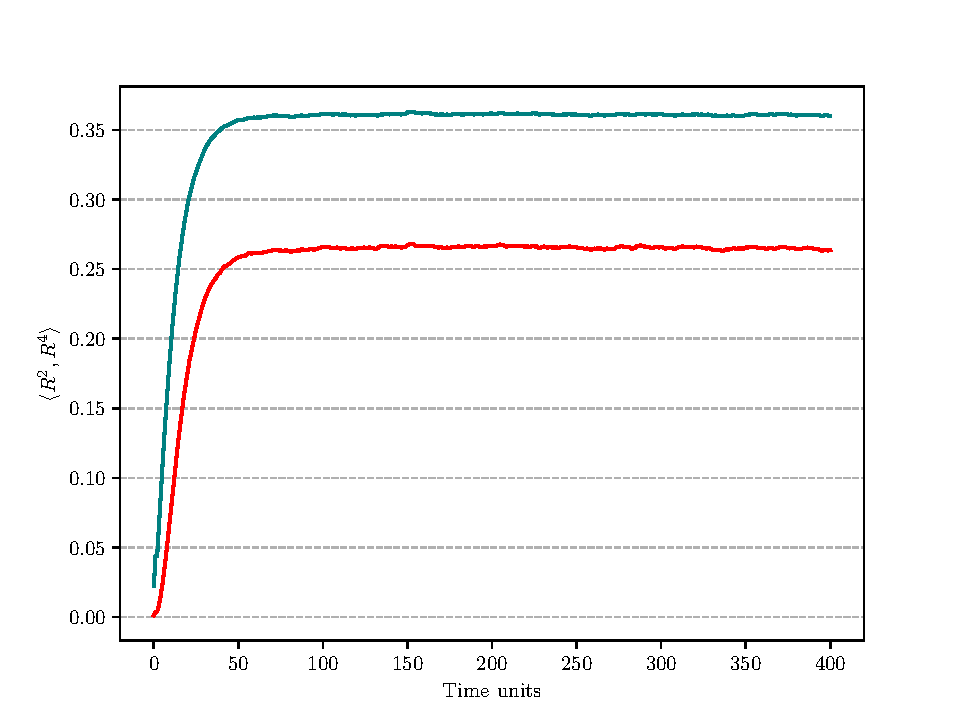
\includegraphics[width=0.75\textwidth]{figs/IKKT_plot.pdf}
	\caption{\label{fig:IKKT_1}The scalar extents for the bosonic IKKT model. After about 200 trajectories, it seems to converge to the answer. 
	The plot is for $N = 200$ ad $\lambda=1$.}
\end{figure}

\begin{equation}
	\langle R^2 \rangle =   \frac{1}{DN} \Bigg \langle \mbox{Tr} \sum_{i=1}^{D} X_{i}^2 \bigg \rangle, 
	~~ \langle R^4 \rangle =   \frac{1}{DN} \Bigg \langle \mbox{Tr} \sum_{i=1}^{D} X_{i}^4 \bigg \rangle, 
\end{equation}
dfsfwef
It is known that $R^2$ should behaves as $\sqrt{\lambda}$ in the large $N$ limit 
from \TODO{Nishimura '98} but we have not found any previous study which fixes the prefactor. Our numerical results suggests that $ \langle R^2 \rangle = 0.361(2) \sqrt{\lambda}$ and $ \langle R^4 \rangle = 0.265(3) \lambda$ with $N = 200$ for a wide range of couplings i.e., 
$\lambda \in [1,100]$. 
One of the standard tests we do for the reliability of the numerical results is 
computing the average action. It can be shown that under a 
change: $X \to e^{\epsilon} X$ if we demand that $Z$ is invariant, 
then we find:

\begin{equation}
\label{eq:SD_IKKT1} 
	\frac{\langle S \rangle}{N^2 - 1} = \frac{D}{4} 
\end{equation}
We show in \TODO{FIg---} that for $D=10$ we get the correct answer and 
hence the reported results above can be fully trusted. 

\begin{mdframed}[backgroundcolor=blue!3] 
	\textsc{} 
	$\bullet$ Exercise (${\star}$): Derive (\ref{eq:SD_IKKT1}) by doing the change: $X_{\mu} \mapsto e^{\epsilon}X_{\mu}$ and ignoring terms in 
	$\mathcal{O}(\epsilon^{2})$
\end{mdframed}


\begin{figure}[htbp] 
	\centering 
	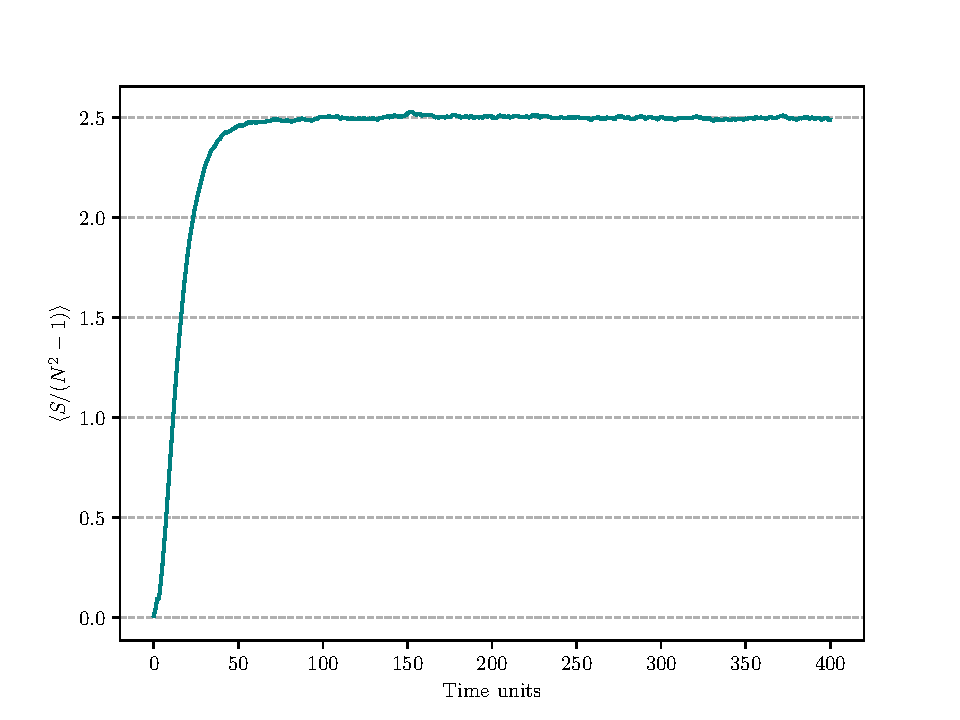
\includegraphics[width=0.75\textwidth]{figs/IKKT_plot_S.pdf}
	\caption{\label{fig:IKKT_2}The average action (normalized) for the $D=10$ bosonic sector of IKKT model.}
\end{figure}


We also note that if we consider $D=3$, then as argued in 
\cite{Hotta:1998en} it becomes little tricky and
\TODO{our results supports this?}. 


There has been some recent work which tries to take the master-field approach to the
IKKT model \cite{Klinkhamer:2021wrv}. This is a promising direction 
but it is not yet clear how effective it will be.  


\vspace{10mm} 

\begin{mdframed}[backgroundcolor=blue!3] 
	\textsc{} 
	$\bullet$ Exercise: Carry out the MC computation for the bosonic IKKT model (10 MM) for the action given in (\ref{eq:IKKT}). After sufficient thermalization cut, check that the results are consistent with exact result obtained using Schwinger-Dyson equations within errors. Refer to appendix for the $\textsc{Python}$ code and to perform Jackknife error analysis with sufficiently large block size. 
\end{mdframed} 


\subsection{BMN matrix model}

We now consider another useful matrix model which is an extesion of the BFSS model. This model is a massive deformation of BFSS (\ref{D0action}) and is known as PWMM (Plane-Wave Matrix Model) 
or BMN after the authors of \cite{Berenstein:2002jq}. The dual descruiptio is on a plane wave background which retains the supersymmetry unlike BFSS which is dual to M-theory o a flat geometry.


\subsubsection{Full sector}

The action reads 
\begin{equation}
	S = S_{\rm{BFSS}} + \frac{N}{4\lambda} \int dt \,\mbox{Tr} \left[
	-\frac{\mu^2}{ 3^2} ( X^i)^2
	-\frac{\mu^2}{ 6^2} (X^a)^2 +
	\frac{\mu}{4}\Psi^\alpha \left(\gamma^{123}\right)_{\alpha \beta} \Psi^\beta 
	- \frac{\sqrt{2}\mu}{3} \epsilon_{ijk} X^iX^jX^k \right] ,
	\label{PWMMaction}
\end{equation}
where the indices $i,j,k$ run over $1,2,3$ and the index $a$ runs over $4,\dots,9$.
The mass parameter $\mu$ breaks the $SO(9)$ global symmetry of (\ref{D0action}) down to $SO(6)\times SO(3)$. 
This mass deformation of BFSS retains maximal supersymmetry \cite{Berenstein:2002jq}.These extra terms in the BMN model gives this model two advantages over the BFSS. 

\begin{itemize}
	\item In the limit of $\mu\to\infty$ the model becomes weakly coupled and can be studied perturbatively usig Gaussian gauged matrix model.  
	\item The mass terms lifts the moduli space of the BFSS model and gives a discrete set of vacua. This is useful for numerical simulations because it means the theory has well-defined thermal canonical ensemble. 
\end{itemize}
However, for a dual gravity description, the mass term which depends on $\mu$ should be small. The lattice coupling will eventually depend on $N, N_{t}, \lambda, \beta, \mu$. The first four should be familiar with BFSS 1d sixteen supercharge lattice coupling, the addition of $\mu$ is what makes the phase structure exciting to study 


\begin{equation}
	S_B = \frac{N}{4\lambda} \sum_{n = 0}^{N_{\tau} - 1} \mbox{Tr} \Bigg[\left(D_{\tau} X_n^i\right)^2 + \sum_{i < j} \left[X_n^i, X_n^j\right]^2 
	+ \left(\frac{\mu}{3} X_n^I\right)^2 + \left(\frac{\mu}{6} X_n^M\right)^2
	+ \frac{\sqrt{2} \mu}{3} \epsilon_{IJK} X_n^I X_n^J X_n^K\Bigg],
\end{equation}
where $N_{\tau}$ is the number of lattice sites. The term which is cubic in scalars is often referred to as `Myers term'. In fact, there exists some studies of model where this term is added to the usual commmutator term.

In those cases, the action becomes:

\begin{equation}
	S = N \mbox{Tr} \Bigg( \sum_{\mu, \nu = 1}^{d > 3} [X_\mu, X_\nu]^2  + \frac{i \alpha}{3} \epsilon^{abc} X_a X_b X_c \Bigg) 
\end{equation}

The bosonic model has a first-order phase transition in the large $N$ limit
For small $\mu$ while for large $\mu$ there is an additional phase transition 
between two confined phases. 


In \cite{Furuuchi:2003sy}, it was claimed that for a model with $d > 1$ 
matrices (bosonic or fermionic), of masses $\omega_{j} > 0$ with $j =
1 . . . d$, the inverse Hagedorn temperature $\beta_{H}$ is given by the solution of:

\begin{equation}
\sum_{j=1}^{d} e^{-\beta_{H} \omega_{j}} = 1. 
\end{equation}


This can be used to accurately determine the critical temperature for the full BMN model at weak couplings. If we define, $\mu/T = x$, the critical temperature is the solution of the following equation:
\begin{equation}
	3e^{-x/3} + 6e^{-x/6} + \underbrace{8e^{-x/4}}_{\text{fermions}}= 1 \implies \frac{T}{\mu} \approx 0.076
\end{equation}


\subsubsection{Bosonic sector}


BMM model has a rich phase structure even with fermions left out. 
It again has a decofinement transition which can be calculated exactly using 


 
This estimate works well also for $ g \to 0$ with no fermions by just removing the term corresponding to fermions above. We compare this exact result to our numerical result and find excellent agreement. 

%T/mu for full model ~ 0.076 can be simply obtained by  doing --> Solve[8 Exp[-x/4] + 
% 3 Exp[-x/3] + 6 Exp[-x/6] == 1, x \[Element] Reals]; to leading order in Mathematica %


In an old work \cite{Mandal:2009vz}, the critical temperature was computed in the large $N$ limit in $1/D$ expansion for the $\mu=0$ couterpart. The result is:

\begin{equation}
T(d) = \frac{\sqrt[3]{d}}{\left(\frac{\frac{203}{160}-\frac{\sqrt{5}}{3}}{d}+1\right) \log (d)}, 
\end{equation}
% T[d_] := d^(1/3)/Log[d]  (1 + 1/d (203/160 - Sqrt[5]/3))^-1; 
It was shown numerically in \cite{Bergner:2019rca}, that for $d = 9$, the obtained $T_{c} = 0.895$ compared well to the analytical result obtained i.e., $T_{c} = 0.894658$. The trasition is first-order. 

In the bosonic BMN case we consider with $d=9$, we must retrieve the above result in the limit $ \mu \to 0$. Therefore, it is expected that the critical temperature will behave as:

\begin{equation}
T_{c} = 0.895 \Big( 1 + f(\mu) \Big)
\end{equation}

We recently perfomed numerical computations and found the form with $N=32,48$. A more ambitious goal would be to compute the $1/D$ expansion with $\mu$. This might be guessed by varying the number of scalar fields i.e., $d \neq 9$. Other thing we can compute is the distribution $\rho$ of eigenvalues of scalars $X$. 
A similar computation can be seen in \cite{Filev:2015hia}. 
 


It is also well-known for BFSS model at high temperatures where the fermions decouple that $ E/N^2 = 6T$ in the notation where $\lambda=1$ and large $N$ limit has been taken. This is a standard result, see \cite{Kawahara:2007ib} for additional details. 

Now, this calculations is not done for mass deformed matrix model such as bosonic BMN. It would be nice to find an expression like one below using our lattice data.

\begin{equation}
\frac{E}{N^2} = 6T \Bigg( 1 + f(\mu) \Bigg)
\end{equation}



\section{Summary}

We have discussed a wide range of matrix models some of which
Are analytically solvable I the plaar limit. 
The purpose is to introduce the reader to Monte Carlo methods and
Show the applications by providing codes and clear explanation. 


\subsection*{Acknowledgements}
The author is indebted to Pedro Vieira
for numerous discussions and for encouragement. 
The author was supported by a postdoctoral fellowship at the Perimeter Institute for 
Theoretical Physics during 2019-2022. Research at Perimeter Institute is supported 
in part by the Government of Canada through the Department of Innovation, Science and 
Economic Development Canada and by the Province of Ontario through 
the Ministry of Economic Development, Job Creation and Trade.
The author would like to thank Department of Science \& Technology, Govern-
ment of India for KVPY (Kishore Vaigyanik Protsahan Yojana) Scholarship during 2008-2010, 
European Union for Erasmus Mundus scholarship during 2010-2011, 
Department of Physics at Syracuse University for support during 2013-2019. 

\newpage 
\appendix


%%%% Appendices now %%%%%
%%%%%%%%%%%%%%%%%%%%%%%%%%%%%%%%%%%%
\section{Character Expansion} 
The method of character expansion is well-known to lattice gauge 
theorists and was first initiated in a seminal work by Migdal \TODO{cite}. 
The basic idea of character expansion is to utilize a specific transform 
on group manifold. The method of character expansion was introduced for 
graph enumeration and solving matrix models in
\cite{DiFrancesco:1992cn, Kazakov:1995ae}. 
This was done since there were many interesting cases 
where the HCIZ formula was not immediately applicable. 
We will consider this method and show how it can be used to solve a 
two Hermitian matrix model with ABAB interaction.
This method has also been applied to dually weighted graphs (DWG). 
\TODO{Check!}. These models have deep connections to the 8-vertex models
in Statistical physics on dynamical planar graphs 
and was also shown to be connected to 
the non-perturbative formulation of three-dimensional Lorentzian quantum gravity \cite{Ambjorn:2001br}.
See \cite{Kazakov:2000aq} for a review of this method. 

Let us consider: 

\begin{equation}
Z = \int \mathcal{D}X \exp \mbox{Tr} \Big[ -X^2 + V(AX) \Big]
\end{equation}
Where $A$ is an external matrix and $V$ is the potential. Because of the general form of the potential HCIZ formula is not applicable. We can do the character expansion as follows:

\begin{equation}
\exp \mbox{Tr} V(AX) = \sum_{R} f_{R} \chi_{R}(AX) 
\end{equation}
Where the coefficients $f_{R}$ are fiction of the irreducible representation 
Of the Gaige group. 

\begin{equation}
f_{R} = \int d\Omega \exp \Big[ \mbox{tTr} V(\Omega)\Big] \chi_{R}(\Omega^\dagger) 
\end{equation}





%%%%%%%%%%%%%%%%%%%%%%%%%%%%%%%%
\section{Orthogonal polynomials}
One of the methods we discussed for the solution of 
large $N$ limit of matrix models was the saddle point approximation. 
However, this method is not useful 
to understand the terms subleading in $1/N$. The method 
of orthogonal polynomials introduced by Bessis \cite{Bessis:1979is} 
is usually used for such computations. In fact, it is also very useful in 
solving multi-matrix models. These polynomials are defined as:

\begin{equation}
	\label{eq:ortho_nn} 
	\int d\lambda e^{-V(\lambda)} P_{n}(\lambda)
	P_{m}(\lambda) = \int d \mu(\lambda) P_{n}(\lambda)
	P_{m}(\lambda) = a_{n} \delta_{mn} 
\end{equation}
where $d \mu(\lambda) = d\lambda e^{-V(\lambda)}$ is the measure  

The basic idea is to rewrite the Vandermonde determinant appearing after we change from matrix basis to the basis of eigenvalues. 

\begin{equation}
	\Delta(\lambda) = \det(\lambda_{i}^{j-1})_{1 \le i, j \le N} = \det(P_{j-1}(\lambda_i))_{1 \le i, j \le N}
\end{equation}


These polynomials can solve:

\begin{equation}
	\label{eq:mm_main}
	\exp(Z) = \int dM \exp[-\mbox{Tr} V(M)] 
\end{equation}

In fact, it can be shown that \ref{eq:mm_main} is equivalent to:

\begin{equation}
	\exp(Z) = N! ~ a_{0}^{N} \prod_{k=1}^{N} f_{k}^{N-k}
\end{equation}

where $f_{k} := a_{k}/a_{k-1}$. Hence, solving the matrix model is now equivalent to solving for the normalization appearing in \ref{eq:ortho_nn}. 

As we have shown in \TODO{....}, we can use this method to solve the unitary matrix model.


%%%%%%%%%%%%%%%%%%%%%%%%%%%%%%%%
\section{Schwinger-Dyson/loop equations}
The basic idea of the loop equations of matrix models is to capture the invariance of the model under field redefinitions. This is also sometimes known as `Schwinger-Dyson (SD) equations'. One of the exercises in the main text was to derive these equations. Here, we will sketch a proof for the interested reader. We start by noting that the integral of the total derivative vanish and hence:

\begin{equation}
	\sum_{i,j} \int dM \frac{\partial}{\partial M_{ij}} \Bigg( (M^k)_{ij}~e^{-N\mathrm{Tr} V(M)}\Bigg) = 0, 
\end{equation}
By computing the derivatives and using large $N$ factorization, we obtain:
\begin{equation}
	\Big< \mathrm{Tr} M^{k} V^{\prime}(M) \Big> = \sum_{l=0}^{k-1} \langle \mathrm{Tr} M^{l} \rangle  \langle \mathrm{Tr} M^{k-l-1} \rangle
\end{equation}
In the steps above, we have used two identities:
\begin{equation}
	\frac{\partial}{\partial M_{ij}} (M^{k})_{ij} = \sum_{l=0}^{k-1} (M^{l})_{ii} (M^{k-l-1})_{jj}
\end{equation}
and, 
\begin{equation}
	\frac{\partial}{\partial M_{ij}} e^{-N\mathrm{Tr} V(M)} = -N V^{\prime}(M)_{ji}~e^{-N\mathrm{Tr} V(M)}
\end{equation}
where $V^{\prime}$ denotes the derivative w.r.t to the matrix. 
However, these loop equations are not valid when the integration is over some other matrix ensembles (such as orthogonal/symplectic). It is better to start from the eigenvalue integral representation to consider general $\beta \in \mathbb{C}$. We can write moments as:

\begin{equation} 
\langle \mbox{Tr} M^k  \rangle = \frac{1}{Z} \int \Delta(\lambda)^{\beta} 
	d\lambda_1 \cdots d\lambda_{N~} \exp\Bigg(-\frac{N\beta}{2} \sum_{i} V(\lambda_{i})\Bigg)  \sum_{i=1}^{N} \lambda_{i}^k
\end{equation}
It is easy to derive `generalized loop equations' from here using the fact that inntegral of total derivatives vanishes. We obtain:

\begin{equation}
		\Big< \mathrm{Tr} M^{k} V^{\prime}(M) \Big> +  \underbrace{k \Bigg(\frac{2}{\beta} - 1 \Bigg) \mathrm{Tr} M^{k-1}}_{\text{zero for $\beta=2$}} = \sum_{l=0}^{k-1} \langle \mathrm{Tr} M^{l} \rangle  \langle \mathrm{Tr} M^{k-l-1} \rangle
\end{equation}

%%%%%%%%%%%%%%%%%%%%%%%%%%%%%

\section{Mathematica code for solution of one-matrix model}

We now give the details to solve the one matrix model in \textsc{Mathematica}. For this we consider the potential:
\[ V(Y) = \frac{Y^2}{2} + \frac{gY^4}{4} \] 
As we have shown in the text, for this case, the higher moments of trace of $Y$ are related and hence we will just calculate $\mbox{Tr}Y^2$ in the planar limit (normalized by $N$). We give the code below for $g=1$. One is encouraged to try and change $g$ and see how the results change.

\begin{mdframed}[backgroundcolor=magenta!1] 
	\begin{footnotesize} 
		\noindent 
		\verb"V[y_]=y^2/2+(g y^4)/4;"\\
		\verb"G[x_]=Integrate[-1/(2\[Pi]I)Sqrt[x^2-a^2]/Sqrt[y^2-a^2](N V'[y])/(x-y),{y,-a,a}," \newline
		\verb"Assumptions->{x>a,a>0}];"\\
		\verb"sol=Series[G[x],{x, \[Infinity], 1}]-N/x//Simplify//Solve[# == 0,a]&//Simplify; "\\
		\verb"Series[G[x],{x,\[Infinity], 5}]//Normal; "\\
		\verb"{Coefficient["\%\verb", x, -3]}/N;"\\
		\%\verb" /. sol;"\\
		\%\verb"/.{g -> 1}//Chop//N// Grid"\\
	\end{footnotesize} 
\end{mdframed}

%%%%%%%%%%%%%%%%%%%%%%%%%%%%

\section{Python code for solution of one-matrix model.}
We now solve the 1MM using the Monte Carlo method which is the 
standard in lattice field theory literature. By executing the code given below
And waiting about 55-60 seconds on a modern laptop, we get the result shown in 
Fig. \ref{fig:F_app1} below. We can readily extend this code (by changing $\texttt{NMAT}$) to study matrix models where the integration is over several different matrices. As we will discuss later, for the case of IKKT model, there are `ten' matrices involved and hence this code will be adjusted accordingly to study that model for given $\lambda$ and $N$. 

\begin{footnotesize} 
\begin{mdframed}[backgroundcolor=magenta!2] 
\begin{footnotesize} 
\begin{lstlisting}[language=Python]
#!/usr/bin/python
# -*- coding: utf-8 -*-

import random
import math
from matplotlib.pyplot import *
from matplotlib import pyplot as plt
import numpy as np
import random
from scipy.linalg import expm
from numpy import linalg as LA
from numpy.linalg import matrix_power
import time 
import datetime 
import sys

startTime = time.time()
print ("STARTED:" , datetime.datetime.now().strftime("%d %B %Y, %H:%M:%S"))

if len(sys.argv) < 4:
  print("Usage:", str(sys.argv[0]), "READIN " " SAVE " " NCOL")
  sys.exit(1)

READIN = int(sys.argv[1])
SAVE = int(sys.argv[2])
NCOL = int(sys.argv[3]) 

NMAT = 1
Niters_sim = 10 # Should be even
g = 1.
dt = 1e-3
nsteps = int(0.5/dt) 
skip = 2.
cut=int(0.25*Niters_sim) 
X = np.zeros((NMAT, NCOL, NCOL), dtype=complex)
mom_X = np.zeros((NMAT, NCOL, NCOL), dtype=complex)
f_X = np.zeros((NMAT, NCOL, NCOL), dtype=complex)
X_bak = np.zeros((NMAT, NCOL, NCOL), dtype=complex)
HAM, expDS, XSQ, X4SQ, X6SQ, MOM = [], [], [], [], [], []

print ("Matrix integral simulation with number of matrices = %4.0f" %(NMAT)) 
print ("NCOL=" "%3.0f " ","  " and 'g' = " " %4.2f" % (NCOL, g)) 
print ("---------------------------------------------------------------------------------")


def dagger(a):
    return np.transpose(a).conj()

def box_muller():  
    PI = 2.0*math.asin(1.0);    
    r = random.uniform(0,1)
    s = random.uniform(0,1)
    p = np.sqrt(-2.0*np.log(r)) * math.sin(2.0*PI*s)
    q = np.sqrt(-2.0*np.log(r)) * math.cos(2.0*PI*s)
    return p,q

def copy_fields(b):
    for j in range(NMAT):
        X_bak[j] = b[j]
    return X_bak

def rejected_go_back_old_fields(a):
    for j in range(NMAT):
        X[j] = a[j]
    return X

def refresh_mom():
    for j in range (NMAT):
        mom_X[j] = random_hermitian()
    return mom_X

def random_hermitian():
    tmp = np.zeros((NCOL, NCOL), dtype=complex)

    for i in range (NCOL):
        for j in range (i+1, NCOL):
            r1, r2 = box_muller()
            tmp[i][i] = complex(r1, 0.0)
            tmp[i][j] = complex(r1, r2)/math.sqrt(2)
            tmp[j][i] = complex(r1, -r2)/math.sqrt(2)

    if np.allclose(tmp, dagger(tmp)):
        return tmp

def hamil(X,mom_X):
    ham = action(X) 
    for j in range (NMAT):
        ham += 0.50 * np.trace(np.dot(mom_X[j],mom_X[j])).real 
    return ham  

def action(X):
    b_action = 0.0 
    for i in range (NMAT):
        b_action += 0.50 * np.trace(np.dot(X[i],X[i])).real   
        b_action += (g/4.0)* np.trace((matrix_power(X[i], 4))).real
    return b_action*NCOL

def force(X): 
    f_X = np.zeros((NMAT, NCOL, NCOL), dtype=complex)
    for i in range (NMAT): 
        f_X[i] = (X[i] + (g*(matrix_power(X[i], 3))))*NCOL
    return f_X

def leapfrog(X,dt):
    mom_X = refresh_mom()
    ham_init = hamil(X,mom_X)

    for j in range(NMAT):
        X[j] += mom_X[j] * dt * 0.5 # Half step 

    for i in range(1, nsteps+1):
        f_X = force(X)
        for j in range(NMAT):
            mom_X[j] -= f_X[j] * dt  # Full step 
            X[j] += mom_X[j] * dt

    f_X = force(X)
    for j in range(NMAT):
        
        mom_X[j] -= f_X[j] * dt
        X[j] += mom_X[j] * dt * 0.5  # Half step 

    ham_final = hamil(X,mom_X)
    return X, ham_init, ham_final

if __name__ == '__main__':


    if READIN ==0:
        for i in range (NMAT): 
            for j in range (NCOL):
                for k in range (NCOL):
                    X[i][j][k] = complex(0.0,0.0) 

    if READIN ==1:
        print ("Reading old config.")
        with open("config_mm.txt") as f2:
            A = np.loadtxt(f2).view(complex)
        f2.close()

        for i in range (NMAT):
            for j in range (NCOL):
                for k in range (NCOL):
                    X[i][j][k] = A[(NCOL*i)+j][k] 

    acc_count = 0
    for MDTU in range (Niters_sim):
        
        X_bak = copy_fields(X) 
        X, start, end = leapfrog(X, dt) 
        change = end - start  
        expDS.append(np.exp(-1.0*change)) 
        if np.exp(-change) < random.uniform(0,1):
            X = rejected_go_back_old_fields(X_bak)
            print(("REJECT: deltaH = " "%8.7f " " startH = " "%8.7f" " endH = " "%8.7f" % (change, start, end)))
        else:   
            print(("ACCEPT: deltaH = " "%8.7f " "startH = " "%8.7f" " endH = " "%8.7f" % (change, start, end)))
            acc_count += 1 

        if MDTU%skip == 0:
            tmp0 = np.trace(np.dot(X[0],X[0])).real
            XSQ.append(tmp0/NCOL)
            tmp1 = np.trace(X[0] @ X[0] @ X[0] @ X[0]).real
            X4SQ.append(tmp1/NCOL)

    if SAVE ==1:

        print ("Saving config.")
        f1 = open("config_mm.txt", "w")
        for i in range (NMAT):
            np.savetxt(f1, X[i].view(float), delimiter= " ")  
        f1.close()

    plt.rc('text', usetex=True)
    plt.rc('font', family='serif')
    MDTU = np.linspace(0, int(Niters_sim/skip), int(Niters_sim/skip), endpoint=True)
    plt.ylabel(r'Tr(X$^2$)',fontsize=16)
    plt.xlabel('Time units', fontsize=16)
    plt.grid(which='major', axis='y', linestyle='--')
    plt.figure(1)
    plot (MDTU, XSQ, 'teal') 
    print ("Fraction of MDTU accepted", (acc_count/Niters_sim)*100) 

    if READIN == 0:
        XSQ = XSQ[cut:]
        X4SQ = X4SQ[cut:]
        X6SQ = X6SQ[cut:]
        expDS = expDS[cut:] 

    print("<Tr X^2 / NCOL>", np.mean(XSQ), "+/-", (np.std(XSQ)/np.sqrt(np.size(XSQ) - 1.0)))
    print("<Tr X^4 / NCOL>", np.mean(X4SQ), "+/-", (np.std(X4SQ)/np.sqrt(np.size(X4SQ) - 1.0)))
    print("exp(-deltaH)", np.mean(expDS), "+/-", np.std(expDS)/np.sqrt(np.size(expDS) - 1.0))
    plt.savefig('mm_plot.pdf') 
    plt.show()
    print ("COMPLETED:" , datetime.datetime.now().strftime("%d %B %Y, %H:%M:%S"))
    endTime = time.time() 
    print ("Running time:", round(endTime - startTime, 2),  "seconds")

\end{lstlisting}
\end{footnotesize} 
\end{mdframed} 
	\end{footnotesize} 
	
\begin{figure}[htbp] 
\centering 
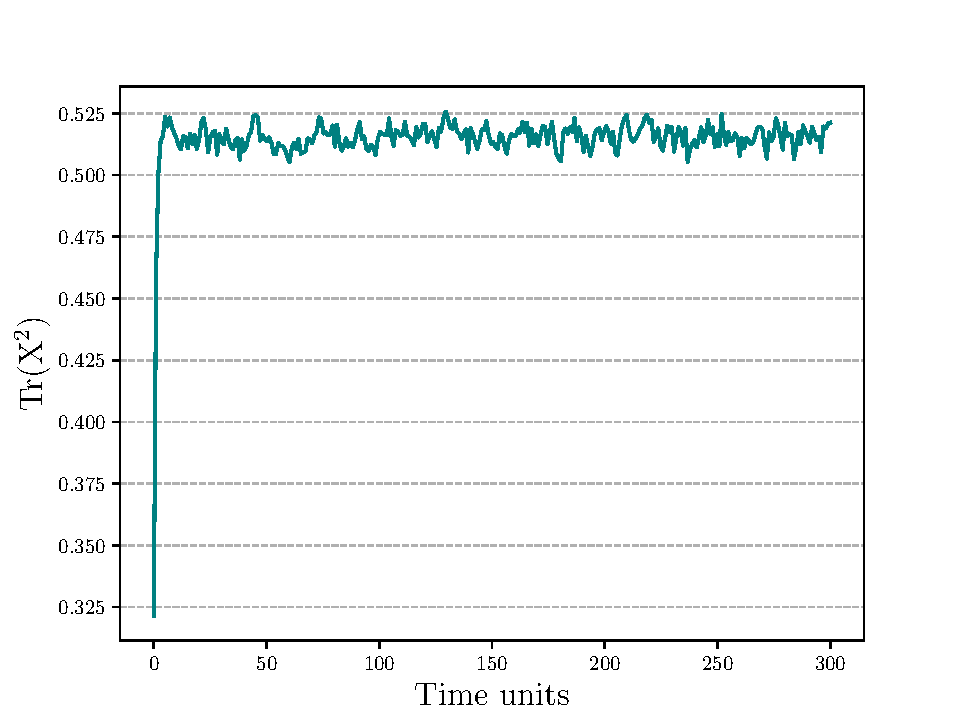
\includegraphics[width=0.75\textwidth]{figs/mm_plot.pdf}
\caption{\label{fig:F_app1}The computed value of $\mbox{Tr}(X^2)$ with MC methods is consistent with that obtained using analytical saddle-point methods. These results are with $N=150$ and $g=1$.}
\end{figure}

%%%%%%%%%%%%%%%%%%%%%%%%%%%%
\section{Bosonic sector of IKKT model: $\textsc{Python}$ code}

We now provide a sketch of the Monte Carlo code with which we can study the bosonic
part of the IKKT model. The details about the model and its relation to the non-perturbative formulations of string theory is discussed in \TODO{SECTion XXX}. 
We have intentionally left out some parts of the code for the reader to fill out from previous study of single matrix model case.  

\begin{footnotesize} 
	\begin{mdframed}[backgroundcolor=magenta!2] 
			%\begin{footnotesize} 
\begin{lstlisting}
#!/usr/bin/python
# -*- coding: utf-8 -*-
import random
import os
import math
from matplotlib.pyplot import *
from matplotlib import pyplot as plt
import numpy as np
import random
from scipy.linalg import expm
from numpy import linalg as LA
import time 
import datetime 
import sys
startTime = time.time()
print ("STARTED:" , datetime.datetime.now().strftime("%d %B %Y %H:%M:%S"))

if len(sys.argv) < 5:
  print("Usage:", str(sys.argv[0]), "READIN " " SAVE_or_NOT " "NCOL " "LAM")
  sys.exit(1)

READIN = int(sys.argv[1])
SAVE = int(sys.argv[2])
NCOL = int(sys.argv[3]) 
LAMBDA = float(sys.argv[4])
COUPLING = float(NCOL/(4.0*LAMBDA))
GENS = NCOL**2 - 1
NSCALAR = 10
dt=5e-4
nsteps = int(1e-2/dt)
Niters_sim=6
GAP=1
xsq = np.zeros((NSCALAR),dtype=float)
X = np.zeros((NSCALAR, NCOL, NCOL), dtype=complex)
mom_X = np.zeros((NSCALAR, NCOL, NCOL), dtype=complex)
f_X = np.zeros((NSCALAR, NCOL, NCOL), dtype=complex)
X_bak = np.zeros((NSCALAR, NCOL, NCOL), dtype=complex)
HAM, expDS, ACT, scalar = [],[],[],[]

print ("IKKT matrix model simulation with only bosonic term")
print ("NCOL=" "%3.0f " ","  " and dimensionless coupling = " " %4.2f" % (NCOL, COUPLING)) 
print ("---------------------------------------------------------------------------------")

def dagger(a):
    return np.transpose(a).conj()

def box_muller():
    PI = 2.0*math.asin(1.0);    
    r = random.uniform(0,1)
    s = random.uniform(0,1)
    p = np.sqrt(-2.0*np.log(r)) * math.sin(2.0*PI*s)
    q = np.sqrt(-2.0*np.log(r)) * math.cos(2.0*PI*s)
    return p,q

def comm(A,B):
    return np.dot(A,B) - np.dot(B,A)

def unit_matrix():
    matrix = np.zeros((NCOL, NCOL), dtype=complex)
    for i in range (NCOL):
        matrix[i][i] = complex(1.0,0.0)
    return matrix

def copy_fields(b):
    for j in range(NSCALAR):
        X_bak[j] = b[j]
    return X_bak

def rejected_go_back_old_fields(a):
    for j in range(NSCALAR):
        X[j] = a[j]
    return X

def refresh_mom():
    for j in range (NSCALAR):
        mom_X[j] = random_hermitian()
    return mom_X

def random_hermitian():
    tmp = np.zeros((NCOL, NCOL), dtype=complex)
    for i in range (NCOL):

        for j in range (i+1, NCOL):
            r1, r2 = box_muller()
            tmp[i][j] = complex(r1, r2)/math.sqrt(2)
            tmp[j][i] = complex(r1, -r2)/math.sqrt(2)

    for i in range (NCOL):
        r1, r2 = box_muller()
        tmp[i][i] = complex(r1, 0.0)
    return tmp 

def kinetic_energy(mom_X):
    s = 0.0 
    for j in range (NSCALAR):
        s += 0.50 * np.trace(np.dot(dagger(mom_X[j]),mom_X[j]))
    return s.real    

def action(X):
    b_action = 0.0 
    for i in range (NSCALAR):
        for j in range (i+1, NSCALAR): 
            co = np.dot(X[i],X[j]) - np.dot(X[j],X[i])
            tr = np.trace(np.dot(co,co))
            b_action -= COUPLING*(tr.real) 
    return b_action

def force(X):
    tmp_X = np.zeros((NSCALAR, NCOL, NCOL), dtype=complex)
    for i in range (NSCALAR): 
        for j in range (NSCALAR):
            if i == j:
                continue 
            else:
                temp = comm(X[i], X[j])
                tmp_X[i] -= comm(X[j], temp)
        f_X[i] = 2.0*COUPLING*dagger(tmp_X[i])
    return f_X 

def leapfrog(X,mom_X, dt):
    for j in range(NSCALAR):
        X[j] += mom_X[j] * dt/2.0
    f_X = force(X)

    for step in range(nsteps):
        for j in range(NSCALAR):
            mom_X[j] -= f_X[j] * dt
            X[j] += mom_X[j] * dt
        f_X = force(X)

    for j in range(NSCALAR):
        mom_X[j] -= f_X[j] * dt
        X[j] += mom_X[j] * dt/2.0
    
    return X, mom_X, f_X

def update(X):
    mom_X = refresh_mom()
    KE = kinetic_energy(mom_X)
    ba = action(X)
    start_act =  ba + KE
    X_bak = copy_fields(X) 
    X, mom_X, f_X = leapfrog(X,mom_X,dt)
    KE = kinetic_energy(mom_X)
    ba = action(X)
    end_act = ba + KE
    change = end_act - start_act
    HAM.append(abs(change))
    expDS.append(np.exp(-1.0*change))   

    if np.exp(-change) < random.uniform(0,1):
        X = rejected_go_back_old_fields(X_bak)
        print(("REJECT: deltaS = " "%8.7f " " startS = " "%8.7f" " endS = " "%8.7f" % (change, start_act, end_act)))
    else:   
        print(("ACCEPT: deltaS = " "%8.7f " "startS = " "%8.7f" " endS = " "%8.7f" % (change, start_act, end_act)))

    ACT.append(ba)

    tmp = 0.0 
    for i in range (0,10):
        val = np.trace(np.dot(X[i],X[i])).real/NCOL
        xsq[i] = val 
        tmp += val 



    tmp /= NSCALAR 
    scalar.append(tmp) 


    if MDTU%GAP == 0:
        f3.write("%4.8f  \n" %(ba/GENS))
        f4.write("%4.8f " "%4.8f " "%4.8f " "%4.8f " "%4.8f " "%4.8f " "%4.8f " "%4.8f " "%4.8f " "%4.8f \n" %(xsq[0],xsq[1],xsq[2],xsq[3],xsq[4],xsq[5],xsq[6],xsq[7],xsq[8],xsq[9]))
    return X


if __name__ == '__main__':


    if READIN ==0:
        for i in range (NSCALAR):  
            X[i] = random_hermitian()/(NCOL**2)  

    if READIN ==1:
        name_f = "config_IKKT/config_IKKT_N{}_l_{}_D_{}.txt".format(NCOL, LAMBDA, NSCALAR)
        if os.path.isfile(name_f) == True: 
            print ("Reading old configuration")
            with open(name_f) as f2:
                A = np.loadtxt(f2).view(complex)
            f2.close()
            for i in range (NSCALAR):
                for a in range (NCOL):
                    for b in range (NCOL):
                        X[i][a][b] = A[(NCOL*i)+a][b] 
        else: 
            print ("Can't find config. file for this NCOL and LAM")
            print ("Starting from fresh")
            for i in range (NSCALAR):  
                X[i] = random_hermitian()

            X = X/(NCOL**2) 


    f3 = open("action_SD.txt", "w")
    f4 = open("extent_of_space_R2.txt", "w")
    for MDTU in range (Niters_sim): 
        X = update(X)
    f3.close()
    f4.close()

    if SAVE ==1:
        print ("Saving config.")
        name_f = "config_IKKT/config_IKKT_N{}_l_{}_D_{}.txt".format(NCOL, LAMBDA, NSCALAR)
        f1 = open(name_f, "w")
        for i in range (NSCALAR):
            np.savetxt(f1, X[i].view(float), delimiter= " ")  
        f1.close()

    ACT = [x/GENS for x in ACT]
    
    print("<S> = ", np.mean(ACT), "+/-", (np.std(ACT)/np.sqrt(np.size(ACT) - 1.0)))
    print("<exp(-deltaH)> = ", np.mean(expDS), "+/-", np.std(expDS)/np.sqrt(np.size(expDS) - 1.0))
    print ("COMPLETED:" , datetime.datetime.now().strftime("%d %B %Y %H:%M:%S")) 
    endTime = time.time() 

    plt.rc('text', usetex=True)
    plt.rc('font', family='serif')
    MDTU = np.linspace(0, Niters_sim, Niters_sim, endpoint=True)
    plt.ylabel(r'$\langle R^2 \rangle$')
    plt.xlabel('Time units')
    plot(MDTU, scalar, 'teal') 
    plt.grid(which='major', axis='y', linestyle='--')
    plt.show()
    plt.ylabel(r'$\langle S/(N^2-1) \rangle$')
    plt.xlabel('Time units')
    plot(MDTU, ACT, 'teal') 
    plt.grid(which='major', axis='y', linestyle='--')
    plt.savefig('IKKT_plot_S.pdf') 
    plt.show()
    print ("Running time:", round(endTime - startTime, 2),  "seconds")
\end{lstlisting}
%\end{footnotesize} 
	\end{mdframed} 
\end{footnotesize}

%%%%%%%%%%%%%%%%%%%%%%%%%%%%
%%%%%%%% Exercises %%%%%%%%%%%%%
%%%%%%%%%%%%%%%%%%%%%%%%%%%%

\section{Solutions to selected Exercises} 

$\bigstar$ Solution to Exercise 5:
\\ \\ 
We want to evaluate: 
\begin{equation}
	\label{eq:sad_sol1} 
	I(\alpha) = \lim_{\alpha \to 0} \int_{-\infty}^{\infty} e^{-\frac{1}{\alpha}f(x)} ~dx, 
\end{equation}
We use the Taylor expansion about the saddle point $x_{0}$ and throw away higher-order terms to get:
\begin{equation}
	\label{eq:sad_sol2}
	f(x) = f(x_{0}) + f^{\prime\prime}(x_{0}) (x-x_0)^{2} + \cdots 
\end{equation}
Using \ref{eq:sad_sol2} in \ref{eq:sad_sol1} along with the famous Gaussian integral result i.e.,  $\int_{-\infty}^{\infty} e^{-\alpha x^2} dx = \sqrt{\frac{\pi}{\alpha}}$ we get the desired result:

\begin{equation}
	\label{eq:sad_sol1} 
	I(\alpha) =  \sqrt{\frac{2\pi \alpha}{f^{\prime\prime}(x_{0})}} e^{-f(x_{0})/\alpha}. 
\end{equation}
To compute the higher order corrections, we have to use the ($\cdots$) in (\ref{eq:sad_sol2}). With some algebra, it is easy to evaluate this. \\ \\ 
\noindent $\bigstar$ Solution to Exercise :
\\ \\ 
We now show that $\det(V) = \prod_{i<j} (\lambda_i - \lambda_j)$ where $V$ is: 
\begin{equation*}
	V = 
	\begin{pmatrix}
		1 & \lambda_1 & \lambda_{1}^{2} & \cdots & \lambda_{1}^{N-1} \\
		1 & \lambda_2 & \lambda_{2}^{2} & \cdots & \lambda_{2}^{N-1} \\ 
		\vdots  & \vdots  & \ddots & \vdots  \\
		1 & \lambda_N & \lambda_{N}^{2} & \cdots & \lambda_{N}^{N-1} 
	\end{pmatrix} = \lambda_{i}^{j-1} 
\end{equation*}

We first note that the determinant is unchanged
if we make the change to all columns except the first given by:

\begin{equation}
	\lambda_{i}^{j-1} \to \lambda_{i}^{j-1} - \lambda_{1} \lambda_{i}^{j-2}
\end{equation}
then we have, 

\begin{equation}
	\det(V^{\prime}) = 
	\begin{vmatrix}
		1 & 0 & 0 & \cdots & 0 \\
		1 & \lambda_2 - \lambda_1 & \lambda_2(\lambda_2 - \lambda_1) & \cdots & \lambda_2^{N-2}(\lambda_2 - \lambda_1) \\ 
		\vdots  & \vdots  & \ddots & \vdots  \\
		1 & \lambda_N - \lambda_1 & \lambda_N(\lambda_N - \lambda_1) & \cdots & \lambda_N^{N-2}(\lambda_N - \lambda_1) \\
	\end{vmatrix}
\end{equation}
By using Laplace Expansion formula for determinants, along the first row we find that $\det(V^{\prime}) = \det(V^{\prime\prime})$ where $V^{\prime\prime}$ is:

\begin{equation}
	\det(V^{\prime\prime}) = 
	\begin{vmatrix}
		 \lambda_2 - \lambda_1 & \cdots & \cdots & \lambda_2^{N-2}(\lambda_2 - \lambda_1) \\ 
		\vdots  & \vdots  & \ddots & \vdots  \\
		\lambda_N - \lambda_1 &  & \cdots &  \lambda_N^{N-2}(\lambda_N - \lambda_1) \\
	\end{vmatrix}
\end{equation}

Taking the factors common in each row, we get:

\begin{equation}
	\det(V) = \det(V^{\prime\prime}) = 
	(\lambda_2 - \lambda_1) \cdots (\lambda_N - \lambda_1)
	\begin{vmatrix}
		1 & \cdots & \cdots & \lambda_2^{N-2} \\ 
		\vdots  & \vdots  & \ddots & \vdots  \\
		1 &  & \cdots &  \lambda_N^{N-2} \\
	\end{vmatrix}
\end{equation}
If we iterate this with this smaller matrix and carry on, we will see that we will get:
\begin{equation}
	\det(V) = \prod_{i<j} (\lambda_j - \lambda_i).
\end{equation}
To define a Vandermonde matrix and compute determinant, we can execute following command in \MA:
\begin{mdframed}[backgroundcolor=magenta!2]
	\begin{footnotesize} 
		\verb"V = Table[Subscript[\[Alpha], i]^j, {i, 1, 5}, {j, 0, 4}];"\\ 
		\verb"Det@V // Simplify"
	\end{footnotesize} 
\end{mdframed}

\noindent $\bigstar$ Solution to Exercise \TODO{...}: 
\\ \\ 
We consider $ X_{\mu} \to (1 + \epsilon) X_{\mu} + \mathcal{O}(\epsilon^2)$
and $\mathcal{D}X \to (1 + \epsilon D (N^2-1))\mathcal{D}X$ with the path integral:

\begin{equation}
Z = \int \mathcal{D}X e^{-S} = \int \mathcal{D}X \exp\Big[-\frac{1}{4g^2} \mbox{Tr} [X_\mu,X_\nu]^2\Big]
\end{equation}
The transformation changes $Z$ by:
\begin{equation}
	Z = Z + \epsilon \Big\{ D(N^2 -1)Z - 4\langle S \rangle Z  \Big\} = Z ( 1 + \epsilon \Big\{ D(N^2 -1) - 4\langle S \rangle   \Big\})
\end{equation}
If we demand that $Z$ remains invariant, the term in the paranthesis should vanish and we get the desired result:

\begin{equation}
	\frac{D}{4} = \frac{\langle S \rangle}{N^2 - 1 }
\end{equation}



\noindent $\bigstar$ Executing following command in \MA will check that Wigner distribution is observed. The deviation from the semi-circle distribution cane be seen for small $n$. \footnote{Please see \texttt{https://www.wolfram.com/language/11/random-matrices} for more}.  

\begin{mdframed}[backgroundcolor=magenta!2]
	\begin{footnotesize} 
		\verb"n = 1000;"\\ 
		\verb"scaledSpectrum=Flatten[RandomVariate[scaledSpectrum\[ScriptCapitalD][n], 100]];"\\
		\verb"Show[Histogram[scaledSpectrum, {0.05}, PDF, ChartStyle -> LightOrange], "  \\ 
		\verb"Plot[PDF[WignerSemicircleDistribution[1], x],{x, -1.5, 1.5}, PlotLegends -> None, " \\
		\verb"PlotStyle -> ColorData[27, 1]], ImageSize -> Medium]"
	\end{footnotesize} 
\end{mdframed}

\noindent $\bigstar$ Solution to Exercise \TODO{XXX}:
\\ \\ Consider (\ref{eq:LE}) with $k=1$, 
    \begin{equation}
    \Big< \mathrm{Tr}\Big(M^{2} + g M^{4}\Big) \Big> = 1 
    \end{equation}
    This then implies, 
     \begin{equation}
     \mathrm{Tr} M^{4} \equiv t_{4} = \frac{1 - \mathrm{Tr} M^{2}}{g} \equiv \frac{1 - t_2}{g} 
     \end{equation}
     We can extend this to $\mathrm{Tr} M^{6} \equiv t_{6}$ which can be obtained in terms of 
     $t_2$ as:  
     
     \begin{equation}
     	t_{6} = \frac{2t_{2} - \frac{(1-t_{2})}{g}}{g}. 
     \end{equation} 

\noindent $\bigstar$ Solution to Exercise 5:
\\ \\  We now show that $ \langle e^{-\Delta H} \rangle = 1$ 
The Hamiltonian of the system is defined as:
\begin{equation}
	H(P,X) = \frac{1}{2}P^2  + S(X)
\end{equation} 

Areas of phase space is preserved i.e.,

\begin{equation}
	dP dX = dP^{\prime} dX^{\prime} 
\end{equation}

Now consider the partition function:

\begin{align}
	\label{eq:ps1} 
	Z &= \int dP^{\prime} dX^{\prime} e^{-H^{\prime} \nonumber }  \\
	&=  \int dP dX e^{-H} e^{H-H^{\prime}}
\end{align}

Dividing (\ref{eq:ps1}) by $Z$ we get, 

\begin{equation}
	\langle e^{H-H^{\prime}} \rangle = 	\langle e^{-\Delta H} \rangle = 1
\end{equation}

$\\ \\$ 
$\bigstar$ Solution to Exercise \TODO{xxx}:
\\ \\  Here we give the code to compute errors using Jacknife method.  
\begin{mdframed}[backgroundcolor=cyan!3] 
	\begin{footnotesize} 
\begin{lstlisting}[language=Python]

#!/usr/bin/python
# -*- coding: utf-8 -*-
#!/usr/bin/python3

import sys
import itertools 
from math import *
data = []; data_tot = 0. ; Data = [] ; data_jack = []

if len( sys.argv ) > 2:
    filename = sys.argv[1]
    therm_cut = int(sys.argv[2])
    blocksize  = int(sys.argv[3])
if len( sys.argv ) <= 2:
    print("NEED 3 ARGUMENTS : filename  therm-cut  blocksize ")
    sys.exit()

file = open(filename, "r")
for line in itertools.islice(file, therm_cut, None):
    
    line = line.split()
    data_i = float(line[0])
    data.append(data_i)
    data_tot += data_i
    n = len(data)

n_b = int(n/blocksize)
B = 0.

for k in range(n_b):
    for w in range((k*blocksize)+1,(k*blocksize)+blocksize+1):
        B += data[w-1]
    Data.insert(k,B)
    B = 0

''' Do the jackknife error estimates '''

for i in range(n_b-1):
    data_jack.append((data_tot - Data[i]) / (n - blocksize))
    data_av = data_tot / n   # Do the overall averages
    data_av = data_av
    data_jack_av = 0.; data_jack_err = 0.
for i in range(n_b-1):
    dR = data_jack[i]
    data_jack_av += dR
    data_jack_err += dR**2

data_jack_av /= n_b-1
data_jack_err /= n_b-1
data_jack_err = sqrt((n_b - 2) * abs(data_jack_err - data_jack_av**2))
print(" %8.7f "  " %6.7f"   " %6.2f" % (data_jack_av, data_jack_err, n_b))

\end{lstlisting}
\end{footnotesize} 
\end{mdframed}

%\newpage 
\bibliographystyle{utphys}
\bibliography{notes1.bib}
\end{document}
